%% Adaptado a partir de :
%%    abtex2-modelo-trabalho-academico.tex, v-1.9.2 laurocesar
%% para ser um modelo para os trabalhos no IFSP-SPO

\documentclass[
    % -- opções da classe memoir --
    12pt,               % tamanho da fonte
    openright,          % capítulos começam em pág ímpar (insere página vazia caso preciso)
    %twoside,            % para impressão em verso e anverso. Oposto a oneside
    oneside,
    a4paper,            % tamanho do papel. 
    % -- opções da classe abntex2 --
    %chapter=TITLE,     % títulos de capítulos convertidos em letras maiúsculas
    %section=TITLE,     % títulos de seções convertidos em letras maiúsculas
    %subsection=TITLE,  % títulos de subseções convertidos em letras maiúsculas
    %subsubsection=TITLE,% títulos de subsubseções convertidos em letras maiúsculas
    % Opções que não devem ser utilizadas na versão final do documento
    %draft,              % para compilar mais rápido, remover na versão final
    MODELO,             % indica que é um documento modelo então precisa dos geradores de texto
    %TODO,               % indica que deve apresentar lista de pendencias 
    % -- opções do pacote babel --
    english,            % idioma adicional para hifenização
    brazil,              % o último idioma é o principal do documento
    pstricks,border=12pt
   ]{ifsp-spo-inf-ctds}
\graphicspath{./anexos}
% ---

% --- 
% CONFIGURAÇÕES DE PACOTES
% --- 
%\usepackage{etoolbox}
%\patchcmd{\thebibliography}{\chapter*}{\section*}{}{}
\usepackage{makecell}
\usepackage{rotating}
\usepackage{lscape}
\usepackage{float}
\usepackage{qrcode}
\usepackage{url}
\usepackage{quoting}

% ---
% Informações de dados para CAPA e FOLHA DE ROSTO
% ---
\titulo{PLATAFORMA INTERCÂMBIO AU PAIR - AUPAMATCH}

% Trabalho individual
%\autor{JOSÉ BRAZ DE ARAÚJO}

% Trabalho em Equipe
% ver também https://github.com/abntex/abntex2/wiki/FAQ#como-adicionar-mais-de-um-autor-ao-meu-projeto
\renewcommand{\imprimirautor}{
\begin{tabular}{lr}
CEZAR GODOY NASCIMENTO	& SP3040755 \\
HENRIQUE OLIVEIRA DE SOUZA & SP3060292 \\
ISABELA SOUZA DUARTE	& SP3030083 \\
JOÃO LUCAS FRANCO FERRAZ LORENA & SP3013529 \\
JONAS ARELLARO CAETANO	& SP3041204 \\
RAFAEL RIBEIRO SANTOS DE CARVALHO	& SP3024008 \\
STEFANY RODRIGUES DOS SANTOS	& SP303027X \\
\end{tabular}
}

\tipotrabalho{Projeto da Disciplina PI1A5}

\disciplina{PI1A5 - Projeto Integrado I}

\preambulo{Trabalho apresentado no curso de Tecnologia em Análise e Desenvolvimento de Sistemas do Instituto Federal de Educação, Ciência e Tecnologia de São Paulo como requisito parcial para a conclusão da disciplina de Projeto Integrado 1.}

\data{\the\year}

% Definir o que for necessário e comentar o que não for necessário
% Utilizar o Nome Completo, abntex tem orientador e coorientador
% então vão ser utilizados na definição de professor
\renewcommand{\orientadorname}{Professor:}
\orientador{JOSÉ BRAZ DE ARAÚJO}
\renewcommand{\coorientadorname}{Professor:}
\coorientador{ANTÔNIO AIRTON PALLADINO}

% ---

% Configurações de aparência do PDF final

% informações do PDF
\makeatletter
    \hypersetup{
            %pagebackref=true,
            pdftitle={\@title}, 
            pdfauthor={\@author},
            pdfsubject={\imprimirpreambulo},
            pdfcreator={LaTeX with abnTeX2},
            pdfkeywords={abnt}{latex}{abntex}{abntex2}{trabalho acadêmico}, 
            colorlinks=true,            % false: boxed links; true: colored links
            linkcolor=blue,             % color of internal links
            citecolor=blue,             % color of links to bibliography
            filecolor=magenta,              % color of file links
            urlcolor=blue,
            bookmarksdepth=4
    }
% --- 

% ---

% ----
% Início do documento
% ----

\begin{document}

    % ---
    % Capa
    % ---
    \imprimircapa

    % Retira espaço extra obsoleto entre as frases.
    \frenchspacing 
    
    \pretextual
    
    % ---
    % Folha de rosto
    % (o * indica que haverá a ficha bibliográfica)
    % ---
    \imprimirfolhaderosto
    %\imprimirfolhaderosto*
    % ---
    
    % Quando registrado na biblioteca
    %
% ---
% Inserir a ficha bibliografica
% ---

% Isto é um exemplo de Ficha Catalográfica, ou ``Dados internacionais de
% catalogação-na-publicação''. Você pode utilizar este modelo como referência. 
% Porém, provavelmente a biblioteca da sua universidade lhe fornecerá um PDF
% com a ficha catalográfica definitiva após a defesa do trabalho. Quando estiver
% com o documento, salve-o como PDF no diretório do seu projeto e substitua todo
% o conteúdo de implementação deste arquivo pelo comando abaixo:
%
% \begin{fichacatalografica}
%     \includepdf{fig_ficha_catalografica.pdf}
% \end{fichacatalografica}
\begin{fichacatalografica}
    \vspace*{\fill}                 % Posição vertical
    \hrule                          % Linha horizontal
    \begin{center}                  % Minipage Centralizado
    \begin{minipage}[c]{12.5cm}     % Largura
    
    \imprimirautor
    
    \hspace{0.5cm} \imprimirtitulo  / \imprimirautor. --
    \imprimirlocal, \imprimirdata-
    
    \hspace{0.5cm} \pageref{LastPage} p. : il. (algumas color.) ; 30 cm.\\
    
    \hspace{0.5cm} \imprimirorientadorRotulo~\imprimirorientador\\
    
    \hspace{0.5cm}
    \parbox[t]{\textwidth}{\imprimirtipotrabalho~--~\imprimirinstituicao,
    \imprimirdata.}\\
    
    \hspace{0.5cm}
        1. Palavra-chave1.
        2. Palavra-chave2.
        I. Orientador.
        II. Universidade xxx.
        III. Faculdade de xxx.
        IV. Título\\            
    
    \hspace{8.75cm} CDU 02:141:005.7\\
    
    \end{minipage}
    \end{center}
    \hrule
\end{fichacatalografica}
% ---


    
    %Caso necessário
    %% ---
% Inserir errata
% ---
\begin{errata}
Elemento opcional da \citeonline[4.2.1.2]{NBR14724:2011}. Exemplo:

\vspace{\onelineskip}


FERRIGNO, C. R. A. \textbf{Tratamento de neoplasias ósseas apendiculares com
reimplantação de enxerto ósseo autólogo autoclavado associado ao plasma
rico em plaquetas}: estudo crítico na cirurgia de preservação de membro em
cães. 2011. 128 f. Tese (Livre-Docência) - Faculdade de Medicina Veterinária e
Zootecnia, Universidade de São Paulo, São Paulo, 2011.

\begin{table}[htb]
\center
\footnotesize
\begin{tabular}{|p{1.4cm}|p{1cm}|p{3cm}|p{3cm}|}
  \hline
   \textbf{Folha} & \textbf{Linha}  & \textbf{Onde se lê}  & \textbf{Leia-se}  \\
    \hline
    1 & 10 & auto-conclavo & autoconclavo\\
   \hline
\end{tabular}
\end{table}

\end{errata}
% ---
    
    %Obrigatório para trabalhos com bancas oficiais
    %% ---
% Inserir folha de aprovação
% ---

% Isto é um exemplo de Folha de aprovação, elemento obrigatório da NBR
% 14724/2011 (seção 4.2.1.3). Você pode utilizar este modelo até a aprovação
% do trabalho. Após isso, substitua todo o conteúdo deste arquivo por uma
% imagem da página assinada pela banca com o comando abaixo:
%
% \includepdf{folhadeaprovacao_final.pdf}
%
\begin{folhadeaprovacao}

  \begin{center}
    {\ABNTEXchapterfont\large\imprimirautor}

    \vspace*{\fill}\vspace*{\fill}
    \begin{center}
      \ABNTEXchapterfont\bfseries\Large\imprimirtitulo
    \end{center}
    \vspace*{\fill}
    
    \hspace{.45\textwidth}
    \begin{minipage}{.5\textwidth}
        \imprimirpreambulo
    \end{minipage}%
    \vspace*{\fill}
   \end{center}
        
   Trabalho aprovado. \imprimirlocal, 24 de novembro de 2012:

   \assinatura{\textbf{\imprimirorientador} \\ Orientador} 
   \assinatura{\textbf{Professor} \\ Convidado 1}
   \assinatura{\textbf{Professor} \\ Convidado 2}
   %\assinatura{\textbf{Professor} \\ Convidado 3}
   %\assinatura{\textbf{Professor} \\ Convidado 4}
      
   \begin{center}
    \vspace*{0.5cm}
    {\large\imprimirlocal}
    \par
    {\large\imprimirdata}
    \vspace*{1cm}
  \end{center}
  
\end{folhadeaprovacao}
% ---

    
    % ---- opcionais 
    % ---
% Dedicatória
% ---
\begin{dedicatoria}
   \vspace*{\fill}
   \centering
   \noindent
   \textit{Dedicamos este trabalho para aqueles que acreditam e lutam pelo sonho de realizar um intercâmbio au pair.}
   \vspace*{\fill}
\end{dedicatoria}
% ---
    %% ---
% Agradecimentos
% ---
\begin{agradecimentos}
Os agradecimentos principais são direcionados à Gerald Weber, Miguel Frasson,
Leslie H. Watter, Bruno Parente Lima, Flávio de Vasconcellos Corrêa, Otavio Real
Salvador, Renato Machnievscz\footnote{Os nomes dos integrantes do primeiro
projeto abn\TeX\ foram extraídos de
\url{http://codigolivre.org.br/projects/abntex/}} e todos aqueles que
contribuíram para que a produção de trabalhos acadêmicos conforme
as normas ABNT com \LaTeX\ fosse possível.

Agradecimentos especiais são direcionados ao Centro de Pesquisa em Arquitetura
da Informação\footnote{\url{http://www.cpai.unb.br/}} da Universidade de
Brasília (CPAI), ao grupo de usuários
\emph{latex-br}\footnote{\url{https://groups.google.com/group/latex-br}} e aos
novos voluntários do grupo
\emph{\abnTeX}\footnote{\url{https://groups.google.com/group/abntex2} e
\url{http://abntex2.googlecode.com/}}~que contribuíram e que ainda
contribuirão para a evolução do \abnTeX.

\end{agradecimentos}
% ---
    %% ---
% Epígrafe
% ---
\begin{epigrafe}
    \vspace*{\fill}
    \begin{flushright}
        \textit{``Não vos amoldeis às estruturas deste mundo, \\
        mas transformai-vos pela renovação da mente, \\
        a fim de distinguir qual é a vontade de Deus: \\
        o que é bom, o que Lhe é agradável, o que é perfeito.''\\
        (Bíblia Sagrada, Romanos 12, 2)}
    \end{flushright}
\end{epigrafe}
% ---
    
    % -- resumo obrigatório
    % ---
% RESUMOS
% ---

% resumo em português
\setlength{\absparsep}{18pt} % ajusta o espaçamento dos parágrafos do resumo
\begin{resumo}
\todo[inline]{fazer o seu resumo, ele só é feito depois que o documento está terminado
\newline
\newline os itens em negrito estão aqui para ressaltar detalhes que devem ser seguidos, mas não se utiliza o negrito em um resumo}

 De acordo com a norma \citetitle{NBR6028:2003} (3.1-3.2) \index{NBR6028}, o resumo\index{resumo} deve ressaltar o contexto, o objetivo, o método, os resultados e as conclusões do documento (portanto deve ser escrito por ultimo). A ordem e a extensão destes itens dependem do tipo de resumo (informativo ou indicativo) e do  tratamento que cada item recebe no documento original. O resumo \textbf{deve ter um paragrafo único} e deve \textbf{ter entre 150 e 500 palavras para trabalhos acadêmicos ou entre 100 e 250 para artigos de periódicos}. O resumo deve ser  precedido da referência do documento, com exceção do resumo inserido no  próprio documento. (\ldots) As palavras-chave devem figurar logo abaixo do resumo, antecedidas da expressão \textbf{Palavras-chave}:, separadas entre si por ponto e finalizadas também por ponto.

 \textbf{Palavras-chaves}: latex. abntex. editoração de texto.
\end{resumo}

% resumo em inglês
\begin{resumo}[Abstract]
 \begin{otherlanguage*}{english}

   This is the english abstract.

\todo[inline]{fazer tradução do resumo, não utilizar tradução automática}

\todo[inline]{Cuidado com termos que só fazem sentido na língua portuguesa, o texto deve ser ajustado para fazer sentido aos leitores que não conhecem a língua portuguesa}

   \vspace{\onelineskip}

   \noindent 
   \textbf{Keywords}: latex. abntex. text editoration.
 \end{otherlanguage*}
\end{resumo}
    
    % ---
    % inserir lista de ilustrações
    % ---
    \pdfbookmark[0]{\listfigurename}{lof}
    \listoffigures*
    \cleardoublepage
    % ---
    
    % ---
    % inserir lista de tabelas
    % ---
    \pdfbookmark[0]{\listtablename}{lot}
    \listoftables*
    \cleardoublepage
    % ---
    
    % ---
    % inserir lista de quadros
    % ---
    \pdfbookmark[0]{\listofquadrosname}{loq}
    \listofquadros*
    \cleardoublepage
    % ---
    % ---
% inserir lista de abreviaturas e siglas
% ATENCAO o SHARELATEX/OVERLEAF GERA O GLOSSARIO SOMENTE UMA VEZ
% CASO SEJA FEITA ALGUMA ALTERAÇÃO NA LISTA DE SIGLAS É NECESSARIO UTILIZAR A OPÇÃO :
% "Clear Cached Files" DISPONIVEL NA VISUALIZAÇÃO DOS LOGS 
% ---
% https://www.sharelatex.com/learn/Glossaries


\ifdef{\printnoidxglossary}{
    \printnoidxglossary[type=\acronymtype,title=Lista de abreviaturas e siglas,style=siglas]
    \cleardoublepage
}{}

    % Definições para lista de siglas

% ATENCAO o SHARELATEX GERA O GLOSSARIO/LISTAS DE SIGLAS SOMENTE UMA VEZ
% CASO SEJA FEITA ALGUMA ALTERAÇÃO NA LISTA DE SIGLAS OU GLOSSARIO É NECESSARIO UTILIZAR A OPÇÃO :
% "Clear Cached Files" DISPONIVEL NA VISUALIZAÇÃO DOS LOGS 
% ---
% https://www.sharelatex.com/learn/Glossaries
%%

\defSigla{abntex}{abnTeX}{ABsurdas Normas para TeX}

\defSigla{capes}{CAPES}{Coordenação de Aperfeiçoamento de Pessoal de Nível Superior}

\defSigla{der}{DER}{Diagrama Entidade Relacionamento}

\defSigla{ibge}{IBGE}{Instituto Brasileiro de Geografia e Estatística}

\defSigla{ifsp}{IFSP}{Instituto Federal de Educação, Ciência e Tecnologia de São Paulo}

\defSigla{jpeg}{JPEG}{Joint Photographic Experts Group}

\defSigla{ldb}{LDB}{Lei de Diretrizes e Bases da Educação Nacional}

\defSigla{mer}{MER}{Modelo Entidade Relacionamento}

\defSigla{se}{SE}{Sigla Exemplo}

\defSigla{sge1}{SGE1}{Sigla Exemplo 1}

\defSigla{sge2}{SGE2}{Sigla Exemplo 2}

\defSigla{suap}{SUAP}{Sistema Unificado de Administração Pública}

\defSigla{ti}{TI}{Tecnologia da Informação}

\defSiglaIngles{ascii}{ASCII}{American Standard Code for Information Interchange}{Código Americano Padrão para Troca de Informações}

\defSiglaIngles{faq}{FAQ}{Frequently asked questions}{Perguntas frequentes}

\defSiglaIngles{poc}{POC}{Proof of Concept}{Prova de Conceito}

\defSiglaIngles{mvp}{MVP}{Minimum Viable Product}{Produto viável mínimo}

\defSiglaIngles{orm}{ORM}{Object Relational Mapping}{Mapeamento Objeto Relacional}

\defSiglaIngles{owasp}{OWASP}{Open Web Application Security Project}{Projeto aberto de segurança para aplicações Web}

\defSiglaIngles{pdf}{PDF}{Portable Document Format}{Formato de Documento Portável}

\defSiglaIngles{png}{PNG}{Portable Network Graphics}{Gráficos Portáveis para Rede}

\defSiglaIngles{qr}{QR}{Quick Response}{Resposta rápida}

\defSiglaIngles{sql}{SQL}{Structured Query Language}{Linguagem de consulta estruturada}

\defSiglaIngles{uml}{UML}{Unified Modeling Language}{Linguagem de Modelagem Unificada}

\defSiglaIngles{url}{URL}{Universal Resource Locator}{Localizador universal de recurso}

\defSiglaIngles{po}{PO}{Product Owner}{Dono do Produto}

\defSiglaIngles{sm}{SM}{Scrum Master}{Mestre do Scrum}

\defSiglaIngles{dt}{DT}{Developers Team}{Time de Desenvolvedores}

\defSiglaIngles{covid}{COVID-19}{Coronavirus Disease 2019}{Diretor Executivo}

\defSiglaIngles{ceo}{CEO}{Chief Executive Officer}{Doença por Coronavírus 2019}

\defSiglaIngles{usa}{USA}{United States of America}{Estados Unidos da América}

\defSiglaIngles{bbc}{BBC}{British Broadcasting Corporation}{Corporação Britânica de Radiodifusão}

\defSiglaIngles{api}{API}{Application Programming Interface}{Interface de Programação de Aplicação}

\defSiglaIngles{aws}{AWS}{Amazon Web Services}{Serviços Web da Amazon}

\defSiglaIngles{css}{CSS}{Cascading Style Sheets}{Folhas de Estilo em Cascata}

\defSiglaIngles{s3}{S3}{Simple Storage Service}{Serviço de Armazenamento Simples}

\defSiglaIngles{ec2}{EC2}{Amazon Elastic Compute Cloud}{Computação em Nuvem Elástica da Amazon}

\defSiglaIngles{spa}{SPA}{Single-page application}{Aplicativo de Página Única}

\defSiglaIngles{html}{HTML}{HyperText Markup Language}{Linguagem de Marcação de HiperTexto}

\defSiglaIngles{svn}{SVN}{Subversion}{Subversão}

\defSiglaIngles{bdd}{BDD}{Behavior Driven Development}{Desenvolvimento Guiado por Comportamento}





    % ---
    % inserir o sumario
    % ---
    \pdfbookmark[0]{\contentsname}{toc}
    \tableofcontents*
    \cleardoublepage
    % ---
    
    % ----------------------------------------------------------
    % ELEMENTOS TEXTUAIS
    % ----------------------------------------------------------
    \textual
    
    \chapter{Introdução}
    % ---
% Capitulo da Introdução
% ---
    O intercâmbio au pair é um programa que oferece a chance de estudar em um país estrangeiro e morar com uma família anfitriã, trabalhando legalmente cuidando das crianças dessa família e recebendo um salário semanal para realizar este serviço. O processo para se tornar au pair tem como base se adequar aos pré-requisitos, como ter determinada idade, possuir experiência comprovada com crianças, entre outros aspectos. Além de preencher os pré-requisitos, em alguns casos se faz necessário passar por uma análise de perfil, que é realizada por uma agência especializada.

    A agência tem o papel de guiar a candidata au pair durante o processo de escolha e aceitação da vaga. Uma au pair pode se cadastrar em diversas agências e tentar se conectar com muitas famílias ao procurar uma vaga na qual o seu perfil se encaixe. Porém, já é possível que a família e a au pair tenham contato através de redes sociais, indicação de outras famílias, entre outros.

    As agências tentam atrair au pairs, destacando os aspectos positivos da experiência como sendo um intercâmbio cultural barato e vantajoso. Segundo anúncio no site Experimento Intercâmbio.
    
    \begin{citacao}
        Se você tem entre 18 e 26 anos, é solteira, gosta de crianças, tem carteira de habilitação, concluiu o ensino médio e tem nível de inglês intermediário, este é o intercâmbio para você. Você será recebida como um membro da família e terá a oportunidade de fazer um curso a sua escolha, enquanto cuida das crianças, vivendo uma nova cultura e praticando o inglês todos os dias! Durante sua estadia nos Estados Unidos, você receberá uma bolsa de estudos e um salário semanal por seu trabalho como au pair. O salário mínimo semanal é calculado pelo Departamento de Estado Americano considerando os custos de moradia e alimentação. As famílias anfitriãs e au pairs são livres para combinar uma remuneração maior do que o mínimo legalmente estabelecido. Além disso, você terá um dia e meio de folga por semana de trabalho e um final de semana livre por mês. Além de 2 semanas de férias no ano. Um sonho essa experiência!
        \cite{experimCultl2022}
    \end{citacao}

    É interessante destacar que o programa é oferecido a jovens que atendam aos pré-requisitos, porém, a maioria das pessoas que realizam este intercâmbio são do sexo feminino, e por isso, em muitos locais encontra-se inclusive a expressão “a au pair” e em muitos sites a linguagem é toda direcionada às mulheres. Por isso, caso o candidato seja do sexo masculino, é importante que ele esteja atento se há essa exigência na vaga.
    
    \begin{citacao}
        O intercâmbio de au pair para homens não é a modalidade mais comum. Por conta disso, nem todas as agências oferecem vagas para homens como au pair no Exterior. Então, antes de mais nada, o candidato tem que procurar alguma agência que ofereça a modalidade deste intercâmbio também para homens. A verdade é que cada vez mais famílias optam por au pair homens para tomar conta de seus filhos.
        \cite{partiuIntercam2022}
    \end{citacao}
    
    As regras de au pair no geral são as mesmas para homens e para mulheres, segundo o site \cite{partiuIntercam2022}, os candidatos e candidatas devem ter inglês entre intermediário e avançado (e isso será comprovado mediante entrevista), deverão ter carteira de habilitação para dirigir carro, ter terminado o ensino médio e disponibilidade de fazer o programa por um ano. Porém, a idade recomendada para as mulheres é entre 18 e 26 anos e para homens, entre de 18 a 27 anos, os homens também precisam comprovar horas de trabalho com crianças (creches, escolas, orfanatos, projetos sociais, filhos de vizinhos, etc), já as mulheres nem sempre há essa exigência, gostar de criança em alguns casos já é suficiente para se adequar aos pré requisitos, e por fim ambos não podem ter filhos.

    O processo para se tornar au pair pode ser cansativo, uma vez que a mesma deve estar sempre atenta a novas publicações de vagas, estando assim à mercê da plataforma da agência e da procura por au pairs por parte das famílias.

    Pensando principalmente na dificuldade de comunicação que esse processo pode acarretar, e em como isso seria prejudicial a todos os envolvidos (au pairs, famílias e agências), pode-se observar que a criação de uma plataforma que visa principalmente a facilitação da comunicação e um consolidado de vagas em um único lugar se faz necessária. 

    A partir dessa observação, o seguinte projeto em desenvolvimento do \href{https://svn.spo.ifsp.edu.br/svn/a6pgp/S202202-PI-NOT/WebbStars}{Grupo 01} (\href{https://webbstarsifspgrupo1.blogspot.com/}{WebbStars}) se propõe a construir uma plataforma que lide com os problemas expostos anteriormente, além de adicionar outras funcionalidades.

    \section{Objetivos}
    
    O projeto elaborado propõe uma solução que atenda au pairs para encontrar famílias anfitriãs. As famílias poderão visualizar o perfil de au pairs que mais se identificou e contatá-las. Por fim, as agências também poderão divulgar os perfis de au pairs e famílias que possuem contrato com a agência. A plataforma tem como objetivo preencher algumas lacunas encontradas na pesquisa de sites para o intercâmbio de au pair, como por exemplo, interligar perfis e facilitar a comunicação, contratação e divulgação de serviços.
    
    Além disso, os custos das principais agências de au pairs não são pequenos. Em muitos casos, é exigido uma inscrição para que o processo de análise de perfil aconteça, as vagas de famílias anfitriãs apareçam e as entrevistas sejam agendadas.
    
    O site \cite{interViagem2022} traz um resumo simplificado do preço de um programa au pair:
    \begin{quadro}[H]
    \centering\footnotesize
    \caption{Resumo simplificado}
    \label{quadro-preco-aupair}
        \begin{tabular}{|p{0.35\linewidth} | p{0.35\linewidth} |}  \hline
        \thead{Descrição} & \thead{Valores} \\
        \hline
        Taxa de entrevistas & \sim R\$400
        \\
        \hline
        Inscrição no programa au pair & A partir de U\$\$500
        \\
        \hline
        Visto (depende do país) / semanal & R\$750 a R\$2000  (Depende do país)
        \\
        \hline
        Passagem (depende do país) & R\$2500 a R\$3500  (Depende do país)
        \\
        \hline
        \textbf{Custos aproximados} & \textbf{R\$7.500,00}
        \\
        \hline
        \textbf{Investimento total de 1 ano} & \textbf{R\$25.300,00}
        \\
        \hline
        \end{tabular}
    \fonte{Valores de Referência - \cite{interViagem2022}}
    \end{quadro}
    
    Em relação ao aspecto financeiro, a preparação de um intercâmbio cultural au pair pode ficar inviável, por isso, o objetivo da plataforma  \href{https://aupamatch.pages.dev/home}{AupaMatch} é que ela tenha baixo custo ou em alguns casos seja gratuita, de fácil manuseio e que contribua para ampla divulgação de perfis das au pair.
    
    A plataforma  pretende contribuir especialmente para ampliar a divulgação de perfis de au pairs e na atuação deste público na comunicação com as famílias anfitriãs, já que tem nas suas características de desenvolvimento maior possibilidade de acesso de au pairs e consequentemente, maior chance de concretizar \gls{match} “encontro”, ou seja, favorecer para que encontros profícuos aconteçam.
    \section{Justificativa}

    O programa de intercâmbio au pair é uma possibilidade de experiência internacional de baixo custo e ampla vivência cultural, social e acadêmica, pois tem no seu desenho original, além da convivência com uma família anfitriã, a possibilidade de aprender a língua do país e há ainda a oportunidade de frequentar um espaço educativo, o que amplia muito a experiência como um todo. 
    
    Por isso, o intercâmbio au pair tem sido considerado vantajoso por muitos jovens que buscam ter experiências culturais no exterior. Além do programa compreender benefícios como custeio de passagens, cursos de idiomas, acomodação, alimentação durante toda a estadia e salários por funções desempenhadas, ainda deve ser considerada a experiência cultural e social que o programa proporciona. 
    
    Diante de uma pesquisa realizada pelo
    \cite{eurekaFacts2020}, que é um site de soluções inteligentes de pesquisa, foi possível mensurar o impacto do programa, pois percebeu-se que os objetivos desejados entre os sujeitos envolvidos têm tido um nível satisfatório.
    
    Foram entrevistados 10.881 participantes de programas au pair e 6.452 famílias anfitriãs, onde constatou-se que:
    
    \begin{itemize}
        \item 97\% das au pairs entrevistadas obtiveram uma melhor compreensão da cultura americana (tradições e costumes);
        \item 90\% das au pairs entrevistadas consideraram excelente (60\%) ou bom (30\%) a experiência que tiveram;
        \item 88\% das au pairs entrevistadas dizem ter melhor compreensão dos valores americanos (liberdade e independência); 
        \item 86\% das famílias anfitriãs entrevistadas dizem manter contato com as participantes mesmo depois da saída do país e fim do programa.
    \end{itemize}
    
    Segundo o site \cite{valorIveste2022}, a pesquisa aponta que o mercado pós crise sanitária da \ac{covid} passa a ter nova demanda de interessados neste programa de intercâmbio. 
    
    \begin{citacao}
       Depois de quase dois anos com viagens canceladas, planos adiados e quebras de contrato, as empresas especializadas em intercâmbio, imigração, vistos e green card começam a ver o mercado voltar a crescer, retomando os patamares de antes da pandemia. (...) “Para 2022 temos uma grande expectativa e projetamos um crescimento bem mais significativo que o do ano passado, principalmente nos serviços de visto e green card para os brasileiros que já estão nos EUA e não pensam em voltar; tanto para aqueles que querem recomeçar no exterior”, comenta Arleth Bandera, a \ac{ceo} da Eagle Intercâmbio.”
       \cite{valorIveste2022}
    \end{citacao}
    
    Diante deste contexto, o mercado de intercâmbio au pair ganha espaço significativamente, e o desenvolvimento de uma plataforma que facilite, amplie e valorize a conexão entre au pairs, famílias anfitriãs e agências expande as oportunidades.
    Ainda com a expansão e crescimento das relações conectadas por meio da internet e o imenso fluxo de pessoas usufruindo e consumindo ferramentas virtuais, surge a necessidade do desenvolvimento de um sistema interligado, alinhado às demandas advindas dos programas de intercâmbio au pair para contribuir e construir novas relações internacionais.
    
    O intercâmbio cultural é um dos desejos mais cobiçados pelos jovens e as ofertas disponíveis no mercado nem sempre são claras e suficientemente simples para proporcionar que este desejo se realize, por conta especialmente do processo de análise e dificuldade de \gls{match} é que se tornar au pair pode ficar mais difícil, a plataforma
    \href{https://aupamatch.pages.dev/home}{AupaMatch} vem para contribuir neste aspecto no sentido de ampliar as ofertas e possibilidades para que o encontro aconteça.

    \section{Análise Comparativa}
    O mercado para o serviço de au pair exige qualificações específicas, pois trata-se de uma atividade sensível e que depende diretamente do índice de intercâmbios bem-sucedidos.
    
    As agências de au pair se destacam pelo índice de aprovação e de confiança das experiências realizadas. 
    Notamos que existem no mercado dois caminhos para a construção de uma boa experiência de au pair.
    
    A primeira delas, seria por meio de interface de uma agência especializada, pois são elas que analisam os perfis tanto das famílias anfitriãs quanto das au pairs. 
    
    Neste caso, a análise de mercado e de concorrência dessa atividade está diretamente ligada ao desempenho das agências e da qualidade das experiências au pairs, das quais se destaca no mercado a agência
    \cite{auPairInAmerica2022}.
    
    Reconhecida como a mais antiga e respeitada agência de au pairs, essa agência será responsável por todo o processo de cadastro, análise, avaliações, documentações, conexões e acompanhamento do intercâmbio.
    
    Numa tradução livre o site da agência \cite{auPairInAmerica2022} diz que “por mais de 30 anos, oferece as melhores oportunidades culturais de cuidados infantis para famílias anfitriãs em todo o país \ac{usa} e au pairs de todo o mundo. Existem outras agências de au pair, mas au pair é o primeiro programa de au pair legal do país, designado pelo governo dos \ac{usa} em 1986”.
    
    O diferencial desta agência está em ser reconhecida pelo governo americano, o que obviamente contribui com a legalidade do serviço, já que parte das atividades do au pair é trabalhar e ser remunerado dentro dos padrões e das leis americanas, aspecto este, que em outros formatos pode trazer complicações, especialmente em relação a questão do visto, que neste caso é todo arranjado pela agência. Obviamente, este serviço de agência de au pair tem um custo ao candidato.
    
    Outro caminho para a construção de uma experiência de intercâmbio au pair, é o oferecido pela plataforma de serviço de \gls{match} entre famílias anfitriãs e au pairs, chamado de
    \cite{auPair.com2022}, trata-se de um site de conexão entre famílias e candidatos au pair diretamente. 
    
    O site da aupair.com diz que ”\cite{auPair.com2022} é uma agência de correspondência online - que é segura e fácil de usar. Como uma plataforma de correspondência online, não podemos participar diretamente do processo de arranjo de au pair, pois não somos uma agência de serviço completo. No entanto, podemos ajudá-lo com informações úteis em nosso site. Se você não quiser organizar sua estadia como au pair, entre em contato com uma de nossas agências de au pair parceiras confiáveis, que irá guiá-lo durante todo o processo e sua estadia como au pair!”
    
    Ou seja, nesta plataforma todos os arranjos são feitos pelos próprios usuários, o site só disponibiliza a possibilidade do próprio au pair realizar todo o processo de encontro da família anfitriã, ou da família anfitriã encontrar diretamente o au pair, sem a interferência de uma agência. Desta forma, todos os trâmites e negociações serão acordados diretamente entre os interessados.
    
    Este serviço também é legalizado, porém, neste formato pode haver situações fora dos padrões e dos controles de qualidade que o serviço de au pair mediado por uma agência oferece e garante. Por exemplo, acordos de remuneração, horas trabalhadas e acompanhamento das atividades durante o intercâmbio. Esta plataforma de \gls{match} au pair é gratuita.
    
    Mesmo com essas diferenças de formatos, estas duas ofertas se destacam no mercado de au pair pela sua atuação e por conta do número de intercâmbios realizados e bem sucedidos, ambas divulgam seus serviços em inglês e por meio de site na internet, os quais exigem inscrição de famílias anfitriãs e au pairs a partir de uma ampla etapa de envio e análise de documentos, entrevistas e qualificações. Essas características dos serviços de ambos os sites transmitem a seriedade e compromisso para que a segurança dos usuários, famílias anfitriãs e candidatos au pair, estejam em primeiro lugar. 
    
    Ambas possuem representação no Brasil, respectivamente pela \cite{experimCultl2022} e pela \cite{centralInter2022}. As duas plataformas disponibilizam potentes possibilidades de encontro e realização de intercâmbio au pair, porém existem características que diferem o formato que o processo será realizado em cada uma delas, e é este o diferencial de cada ferramenta. A possibilidade da autonomia proposta em um deles é interessante, mas expõe os usuários a uma experiência fora dos padrões, pois por ser concretizado os acordos diretamente entre os interessados, não há manutenção externa ou controle de qualidade.
    
    Segundo reportagem da \ac{bbc}, este serviço tem sido interpretado como a “escravidão moderna”, pois há um disparate em relação aos valores e acordos que tem sido firmados e legislação trabalhista vigente \cite{bbcNewsBrasil2017}.
    
    Já no formato onde a agência coordena as tramitações, além do custo, os interessados estarão sujeitos às exigências e acordos pré-estabelecidos, porém é dessa forma que a alta qualidade do encontro de au pairs e famílias anfitriãs será garantido.
    
    A proposta de aplicação web terá uma atuação diferenciada dos serviços oferecidos nestes dois formatos apresentados, pois a plataforma tem como objetivo ampliar as ofertas de todos os sujeitos envolvidos no contexto au pair, quais sejam: famílias anfitriãs, agências e candidatos au pairs.
    
    O \autoref{quadro-analise-de-mercado} a seguir ilustra nossa análise da concorrência:
        \begin{quadro}[H]
        \caption{Análise da Concorrência}
        \label{quadro-analise-de-mercado}
        \small
        \begin{tabular}{|l|c|c|c|}
        \hline
        \textbf{Funcionalidades} & \multicolumn{1}{l|}{\textbf{Au Pair in América}} & \multicolumn{1}{l|}{\textbf{AuPair.com}} & \multicolumn{1}{l|}{\textbf{AupaMatch}} \\ \hline
        
        Gerenciador de usuário               & \circlemark & \circlemark & \circlemark \\ \hline
        Identificar e autenticar com usuário & \circlemark & \circlemark & \circlemark \\ \hline
        Definir perfil de usuário            & \circlemark & \circlemark & \circlemark \\ \hline
        Gerenciador de anúncio de vaga       &   &   & \circlemark \\ \hline
        Aplicar candidatura em vagas         &   &   & \circlemark \\ \hline
        Salvar vagas em favoritos            &   & \circlemark & \circlemark \\ \hline
        Consolidar vagas                     &   &   & \circlemark \\ \hline
        Filtro de busca                      &   &   & \circlemark \\ \hline
        Priorização e vagas                  &   &   & \circlemark \\ \hline
        \end{tabular}
        \fonte{Autores}
        \end{quadro}

    
    \chapter{Revisão da Literatura}
    % ---
% Capitulo de revisão de literatura
% ---

    Fundado em 1986, o programa de au pair nos \ac{usa} começou como um programa de diplomacia. Desde então, cresceu e se tornou algo muito maior. É uma forma de difundir a tolerância e compreensão intercultural. É uma chance de construir laços com pessoas de todas as esferas da vida. É uma oportunidade dos jovens se tornarem cidadãos globais, modelos e embaixadores de países próximos e distantes \cite{culturalCare2022}.
    
    Au pair é uma expressão da língua francesa que significa ``ao par'' ou ''igual'' e tem como origem a ideia de equilíbrio econômico entre serviços trocados. No mundo todo a expressão au pair é utilizada para definir jovens estrangeiros que participam de um programa de intercâmbio cultural, onde em troca de cuidar das crianças da família recebe uma bolsa de estudos e moradia.
    
    São muitos os tipos de intercâmbios culturais possíveis, algumas alternativas vão desde trabalhos voluntários até estágios remunerados, ou a possibilidade de ser au pair cuidando de idosos. Há também a possibilidade  no mercado de intercâmbio para os mais jovens de cursar o ensino médio em escolas renomadas dos \ac{usa} e ter uma experiência de intercâmbio cultural, esse formato é o famoso \gls{high-school} no \ac{usa} \cite{stbAuPair2022}.

    \section{Experiência au pair}

    Nas plataformas de programas au pairs mais seguras e confiáveis disponíveis no mercado, há lacunas a serem preenchidas em relação principalmente a comunicação e de perfis au pairs dentro deste contexto de intercâmbio.
    
    A construção de uma plataforma que somasse e que contribuísse no processo complexo que o intercâmbio au pair exige partiu de dois sites: \cite{auPair.com2022} e \cite{auPairInAmerica2022}.
    Ambos com mais de 20 anos de experiência no mercado au pair. Porém, outros veículos forneceram novas interpretações do programa de intercâmbio au pair, por exemplo o \cite{bbcNewsBrasil2017} que trouxe uma interpretação do ponto de vista econômico do programa, e traz uma provocação em relação ao custo benefício e a exploração do trabalho. 
    
    Outros aspectos específicos desse tipo de intercâmbio cultural podem ser encontrados e esclarecidos em sites brasileiros consolidados no mercado de intercâmbio, como o \cite{partiuIntercam2022}, \cite{interViagem2022}, que traz dados concretos de custos de programas au pairs, o \cite{culturalCare2022}, com informações gerais, \cite{eurekaFacts2020} com pesquisas de mercado, além das duas plataformas que representam os dois sites norte americanos mais respeitados no mercado, que são \cite{experimCultl2022} e \cite{centralInter2022}. A construção do entendimento da dimensão do significado e da seriedade do intercâmbio cultural com as características au pair foi sendo concebida em torno de diversas referências, e que fundamentalmente compuseram a visão geral do programa.
    
    \section{A importância da internet no mercado au pair}
    
    Há muitos sites na internet que oferecem informações em relação ao programa de intercâmbio au pair. É necessário verificar as fontes para constatar a procedência de seus conteúdos e comprovar se são realmente verdadeiras. Não há outra forma de construir o caminho de intercâmbio cultural au pair que não seja por meio da internet, mesmo as agências trabalhando em torno de alimentar os perfis tanto das au pairs quanto das famílias por meio de seus sites.
   
    O site \cite{auPair.com2022}, referência fundamental para este tipo de intercâmbio deixa claro que há muitas empresas mal-intencionadas e que a candidata ao programa de intercâmbio au pair, deve em qualquer situação entrar em contato com as autoridades legais ou embaixadas do país de destino para confirmar tanto as informações do programa de au pair quanto às informações em relação ao visto de permanência no país.
    Outra importante informação em relação ao visto de permanência é que em algumas situações, há o estímulo para que a candidata utilize outro tipo de visto de permanência que não o de trabalho, o site \cite{auPair.com2022} é categórico quando diz
    
    \begin{citacao}
    Responda NÃO aos que lhe pedem para se tornar seu au pair com um visto de turista de 6 meses ou apenas com um ESTA, que só é válido por até 3 meses! Isto é ilegal! Assim que você atravessar a fronteira dos EUA, você será enviado de volta ao seu país! O programa au pair pode variar de acordo com as regulamentações do país anfitrião. A e o au pair e a família anfitriã devem verificar quais são os requisitos que devem ser cumpridos. Recomendamos que as e os au pairs escolham um país e leiam os requisitos gerais para se tornarem au pair. Se a e o au pair precisar de um visto para o país anfitrião, a embaixada do país anfitrião - localizada no país de residência da ou do au pair - decidirá se a pessoa é elegível para obter o visto. 
    \cite{auPair.com2022}
    \end{citacao}
    
    Mesmo assim, as plataformas digitais ainda são as maiores fontes de informações em relação ao programa de intercâmbio au pair e elas trazem benefícios pela rapidez e facilidade de acesso às informações e pela possível pesquisa por parte das candidatas ao programa au pair em confirmar a idoneidade das empresas divulgadas na internet.
    É interessante destacar que as empresas mais sérias, propõem sempre que um \textbf{contrato} seja estabelecido entre as partes, e há alguns pontos de atenção fundamentais a serem pesquisadas pelas candidatas em relação a isso, segundo o site \cite{auPair.com2022} o fundamental é que este contrato deve conter, como demonstrado abaixo:

    \begin{quadro}[H]
    \centering\footnotesize
    \caption{Estrutura de contrato au pair}
    \label{quadro-contrato-aupair}
        \begin{tabular}{|p{0.32\linewidth} | p{0.62\linewidth} |}  \hline
        \thead{Descrição} & \thead{Detalhes} \\
        \hline
        Duração da estadia & Quanto tempo a estadia durará?
        \\
        \hline
        Data de início e fim do contrato & Quando a estadia da/do au pair vai começar? Quando vai terminar? 
        \\
        \hline
        Pagamento mensal / semanal & Quanto a au pair ganhará em troca do serviço fornecido?
        \\
        \hline
        Férias & Quantos dias livres a/o au pair terá e quando?  
        \\
        \hline
        Acomodações e refeições & Onde vai morar a au pair? Descrever o quarto da/do au pair, regras gerais, etc. 
        \\
        \hline
        Horas de trabalho & Quantas horas a au pair deve trabalhar? Qual será o horário de trabalho?  
        \\
        \hline
        Despesas de transporte no exterior & Quem vai cobrir as despesas de transporte no país de acolhimento? A au pair terá o direito de usar o carro da família? A au pair receberá um cartão mensal de transporte?  
        \\
        \hline
        Seguro & Quem será responsável pelo seguro médico da/do au pair? A au pair terá algum seguro extra (responsabilidade, acidente, etc.)?  
        \\
        \hline
        Responsabilidades de au pair & Quais serão os deveres da/ do au pair durante sua estadia?  
        \\
        \hline
        Despesas de viagem & Quem vai pagar as despesas da viagem da au pair para chegar ao País Anfitrião?  
        \\
        \hline
        Cancelamento de contrato & Qual é o prazo de aviso prévio em caso de cancelamento do contrato?
        \\
        \hline
        Custos do visto & Quem vai pagar pelas despesas do visto?
        \\
        \hline
        \end{tabular}
    \fonte{Site: \cite{auPair.com2022}}
    \end{quadro}
    
    Com essas plataformas virtuais verificadas e avaliadas pelos envolvidos no processo de candidatura au pair, com uma pesquisa intensa em relação às vagas, as ferramentas e possibilidades de intercâmbio, uma experiência au pair de intercâmbio cultural positiva é possível e são muitos os relatos e as histórias de sucesso divulgadas nas redes, algumas com extrema sinceridade.
    
    \begin{citacao}
    Ficamos muito felizes com a plataforma vindo de uma experiência negativa com outra plataforma (apesar de termos pago, não conseguimos encontrar nenhuma au pair disponível). Muito úteis são as funções que mostram o nível de atividade da au pair. Esta foi nossa primeira experiência com um aupair que terminou há uma semana. A experiência foi positiva, embora esperássemos mais entusiasmo e participação em atividades familiares por parte da au pair. Se repetirmos a experiência no futuro, definiremos melhor as regras da casa, especialmente no que diz respeito à limpeza do uso exclusivo da au pair.
    \cite{auPair.com2022}
    \end{citacao}
    
    Portanto é necessário destacar a necessidade de ampliação da oferta de divulgação de perfis au pairs para aumentar as chances de soluções para que encontros entre famílias anfitriãs e au pairs aconteçam com maior frequência, segurança e conforto.

    \chapter{Metodologia de Gestão e Desenvolvimento
    do Projeto}
    % ---
% Capitulo da Metodologia de Gestão e Desenvolvimento do Projeto
% ---
  Devido às características do projeto e da equipe, optou-se por utilizar as práticas do framework ágil \gls{scrum}. 

\section{Organização da Equipe}
As atividades foram divididas de acordo com o conhecimento técnico e habilidade. O \autoref{papeis} indica os papéis de cada membro da equipe.

\begin{quadro}[H]
	\centering\footnotesize
    \ABNTEXfontereduzida
    \caption{Papéis}
    \label{papeis}
    \resizebox {1 \textwidth }{!}{
        \begin{tabular}{|l|c|c|c|c|c|c|c|}
            \hline
            \thead{Papéis} & \thead{Cezar} & \thead{Henrique} & \thead{Isabela} & \thead{João} & \thead{Jonas} & \thead{Rafael} & \thead{Stefany} \\
            \hline
            PO &        &         &  \circlemark     &        &         &     &      \\
            \hline
            SM & \circlemark       &          &       &         &      &     &\\
            \hline
            DT & \circlemark       & \circlemark        &  \circlemark     &  \circlemark      & \circlemark        & \circlemark    &  \circlemark \\   
            \hline
        \end{tabular}
    }
\fonte{Autores}
\end{quadro}

\begin{itemize}
    \item \textbf{\ac{po}} é a \textbf{Isabela Souza Duarte}, responsável por definir as \gls{histórias de usuário} e priorização do \emph{\gls{backlog}} da equipe.
    \item \textbf{\ac{sm}} é o \textbf{Cezar Godoy Nascimento}, responsável por auxiliar o \ac{po} e a cumprir prazos de \gls{sprints}, priorizar itens do \emph{\gls{product-backlog}} e condenar as \emph{\gls{dailys}}.
    \item \textbf{\ac{dt}} - Cada integrante é responsável por determinada atividade para o desenvolvimento do projeto, desde a idealização do projeto e implementação de toda arquitetura proposta, infraestrutura, \emph{\gls{back-end}} e \emph{\gls{front-end}} da aplicação, garantindo assim o cumprimento dos requisitos do projeto. 
    O \autoref{divisao-atividade} aborda as distribuições das atividades.
\end{itemize}


\begin{quadro}[H]
	\centering\footnotesize
    \ABNTEXfontereduzida
    \caption{Distribuição de Atividades}
    \label{divisao-atividade}
    \resizebox {1 \textwidth }{!}{
        \begin{tabular}{|l|c|c|c|c|c|c|c|}
            \hline
            \thead{Atividade} & \thead{Cezar} & \thead{Henrique} & \thead{Isabela} & \thead{João} & \thead{Jonas} & \thead{Rafael} & \thead{Stefany} \\
            \hline
            Back-End &    \circlemark    &   \circlemark       &       &  \circlemark       &         &     &      \\
            \hline
            Blog & \circlemark       &  \circlemark        & \circlemark      &  \circlemark       &  \circlemark       &  \circlemark    & \circlemark     \\
            \hline
            Quadro Kanban & \circlemark       &  \circlemark        & \circlemark      &  \circlemark       &  \circlemark       &  \circlemark    & \circlemark     \\
            \hline
            Backlog & \circlemark       &          &  \circlemark     &       &        &      &      \\
            \hline
            Banco de Dados &   \circlemark   &  \circlemark        &       &   \circlemark      &         &     &   \\
            \hline
            Documentação e Modelagem & \circlemark       &  \circlemark        & \circlemark      &  \circlemark       &  \circlemark       & \circlemark     &  \circlemark   \\
            \hline
            Front-End &        &          &  \circlemark     &         &         & \circlemark    & \circlemark   \\
            \hline
            Vídeos &       &          &       &         &   \circlemark      &  \circlemark    &     \\
            \hline
        \end{tabular}
    }
\fonte{Autores}
\end{quadro}

\section{Gestão do Tempo}
As cerimônias ocorrem durante as \gls{sprints}. É de suma importância a participação dos \ac{dt}. Pois, é necessário para termos uma visão melhor de como anda o andamento das atividades da equipe. Portanto, observe o tempo de cada cerimônia abaixo:
\begin{itemize}
    \item \textbf{Sprint:} Duração de 7 dias;
    \item \textbf{Planejamento da Sprint:} Duração de 2 horas;
    \item \textbf{\emph{Daily} Scrum:} Duração de 15 minutos;
    \item \textbf{\emph{Review:}} Duração de 30 minutos;
    \item \textbf{Retrospectiva da Sprint:}  Duração de 1 hora;
\end{itemize}
\subsection{Sprints}
O andamento das tarefas é acompanhado nas \emph{\gls{dailys}} e no \emph{\gls{board}} do GitHub Projects onde é organizado e priorizado as atividades do projeto. O \autoref{andamento-tarefas} mostra todas as \gls{sprints} e seu determinado objetivo.

\begin{quadro}[H]
\centering\footnotesize
\caption{Sprints}
\label{andamento-tarefas}
        \begin{tabular}{|p{0.25\linewidth} | p{0.10\linewidth} | p{0.60\linewidth} |}  \hline
        \thead{Sprints} & \thead{Duração} & \thead{Objetivo} \\
        \hline
        Sprint 1 - 09/08 ao 15/08 & 7 dias &   Definição da proposta, criação do blog, canal no Youtube, github e \ac{svn}.
        \\
        \hline
        Sprint 2 - 16/08 ao 22/08 & 7 dias & Estruturação da documentação inicial e apresentação da proposta. 
        \\
        \hline
        Sprint 3 - 23/08 ao 29/08 & 7 dias & Elicitação de \gls{requisitos-funcionais}, \gls{requisitos-nao-funcionais}, \gls{histórias de usuário} e \gls{modelagem}.
        \\
        \hline
        Sprint 4 - 30/08 ao 05/09 & 7 dias & Correção da documentação baseada no feedback dos professores.  
        \\
        \hline
        Sprint 5 - 06/09 ao 12/09 & 7 dias & Finalização de ajustes na documentação e entrega do desenho da aplicação.  
        \\
        \hline
        Sprint 6 - 13/09 ao 19/09 & 7 dias & Ajustes na documentação do desenho da aplicação solicitados pelos professores e continuação no desenvolvimento do \ac{der} e o \ac{mer}.  
        \\
        \hline
        Sprint 7 - 20/09 ao 26/09 & 7 dias & Desenvolvimento e entrega da apresentação do desenho da aplicação.  
        \\
        \hline
        Sprint 8 - 27/09 ao 03/10 & 7 dias & Inicialização da \ac{poc}, criação do \gls{front-end} e \gls{back-end}.  
        \\
        \hline
        Sprint 9 - 04/10 ao 10/10 & 7 dias & Andamento do desenvolvimento da \ac{poc}.  
        \\
        \hline
        Sprint 10 - 11/10 ao 17/10 & 7 dias & Finalização e entrega da \ac{poc}.  
        \\
        \hline
        Sprint 11 - 18/10 ao 25/10 & 7 dias & Finalização da documentação e desenvolvimento do \ac{mvp}. 
        \\
        \hline
        Sprint 12 - 26/10 ao 01/11 & 7 dias & Finalização e entrega da documentação e desenvolvimento do \ac{mvp}. 
        \\
        \hline
        Sprint 13 - 02/11 ao 08/11 & 7 dias & Finalização e entrega da documentação e desenvolvimento do \ac{mvp}. 
        \\
        \hline
        Sprint 14 - 09/11 ao 15/11 & 7 dias & Realização de melhorias do \ac{mvp}. 
        \\
        \hline
        Sprint 15 - 16/11 ao 22/11 & 7 dias & Apresentação do \ac{mvp}. 
        \\
        \hline
        Sprint 16 - 23/11 ao 29/11 & 7 dias & Apresentação do \ac{mvp}. 
        \\
        \hline
        Sprint 17 - 30/11 ao 06/12 & 7 dias & Realizar ajustes de entregar versão final da documentação  do \ac{mvp}. 
        \\
        
        
        \hline
        \end{tabular}
\fonte{Autores}
\end{quadro}

\section{Ferramenta de Gerenciamento do Projeto}
\begin{itemize}
    \item \textbf{GitHub Projects:} Foi utilizada a ferramenta do GitHub Projects, o qual destina-se para o gerenciamento de equipes, o qual permite listar as tarefas que devemos realizar na semana e consequentemente da visualização do status de cada tarefa no \emph{\gls{board}}.
\end{itemize}

\section{Ferramentas para Comunicação da Equipe}
\begin{itemize}

    \item \textbf{Whatsapp e Google Meet:} As ferramentas foram utilizadas com o propósito de realizar as reuniões da equipe e alinhamento das atividades.
\end{itemize}
    
    \chapter{Desenvolvimento do Projeto}
    % ---
% Capitulo da Introdução
% ---
    O intercâmbio au pair é um programa que oferece a chance de estudar em um país estrangeiro e morar com uma família anfitriã, trabalhando legalmente cuidando das crianças dessa família e recebendo um salário semanal para realizar este serviço. O processo para se tornar au pair tem como base se adequar aos pré-requisitos, como ter determinada idade, possuir experiência comprovada com crianças, entre outros aspectos. Além de preencher os pré-requisitos, em alguns casos se faz necessário passar por uma análise de perfil, que é realizada por uma agência especializada.

    A agência tem o papel de guiar a candidata au pair durante o processo de escolha e aceitação da vaga. Uma au pair pode se cadastrar em diversas agências e tentar se conectar com muitas famílias ao procurar uma vaga na qual o seu perfil se encaixe. Porém, já é possível que a família e a au pair tenham contato através de redes sociais, indicação de outras famílias, entre outros.

    As agências tentam atrair au pairs, destacando os aspectos positivos da experiência como sendo um intercâmbio cultural barato e vantajoso. Segundo anúncio no site Experimento Intercâmbio.
    
    \begin{citacao}
        Se você tem entre 18 e 26 anos, é solteira, gosta de crianças, tem carteira de habilitação, concluiu o ensino médio e tem nível de inglês intermediário, este é o intercâmbio para você. Você será recebida como um membro da família e terá a oportunidade de fazer um curso a sua escolha, enquanto cuida das crianças, vivendo uma nova cultura e praticando o inglês todos os dias! Durante sua estadia nos Estados Unidos, você receberá uma bolsa de estudos e um salário semanal por seu trabalho como au pair. O salário mínimo semanal é calculado pelo Departamento de Estado Americano considerando os custos de moradia e alimentação. As famílias anfitriãs e au pairs são livres para combinar uma remuneração maior do que o mínimo legalmente estabelecido. Além disso, você terá um dia e meio de folga por semana de trabalho e um final de semana livre por mês. Além de 2 semanas de férias no ano. Um sonho essa experiência!
        \cite{experimCultl2022}
    \end{citacao}

    É interessante destacar que o programa é oferecido a jovens que atendam aos pré-requisitos, porém, a maioria das pessoas que realizam este intercâmbio são do sexo feminino, e por isso, em muitos locais encontra-se inclusive a expressão “a au pair” e em muitos sites a linguagem é toda direcionada às mulheres. Por isso, caso o candidato seja do sexo masculino, é importante que ele esteja atento se há essa exigência na vaga.
    
    \begin{citacao}
        O intercâmbio de au pair para homens não é a modalidade mais comum. Por conta disso, nem todas as agências oferecem vagas para homens como au pair no Exterior. Então, antes de mais nada, o candidato tem que procurar alguma agência que ofereça a modalidade deste intercâmbio também para homens. A verdade é que cada vez mais famílias optam por au pair homens para tomar conta de seus filhos.
        \cite{partiuIntercam2022}
    \end{citacao}
    
    As regras de au pair no geral são as mesmas para homens e para mulheres, segundo o site \cite{partiuIntercam2022}, os candidatos e candidatas devem ter inglês entre intermediário e avançado (e isso será comprovado mediante entrevista), deverão ter carteira de habilitação para dirigir carro, ter terminado o ensino médio e disponibilidade de fazer o programa por um ano. Porém, a idade recomendada para as mulheres é entre 18 e 26 anos e para homens, entre de 18 a 27 anos, os homens também precisam comprovar horas de trabalho com crianças (creches, escolas, orfanatos, projetos sociais, filhos de vizinhos, etc), já as mulheres nem sempre há essa exigência, gostar de criança em alguns casos já é suficiente para se adequar aos pré requisitos, e por fim ambos não podem ter filhos.

    O processo para se tornar au pair pode ser cansativo, uma vez que a mesma deve estar sempre atenta a novas publicações de vagas, estando assim à mercê da plataforma da agência e da procura por au pairs por parte das famílias.

    Pensando principalmente na dificuldade de comunicação que esse processo pode acarretar, e em como isso seria prejudicial a todos os envolvidos (au pairs, famílias e agências), pode-se observar que a criação de uma plataforma que visa principalmente a facilitação da comunicação e um consolidado de vagas em um único lugar se faz necessária. 

    A partir dessa observação, o seguinte projeto em desenvolvimento do \href{https://svn.spo.ifsp.edu.br/svn/a6pgp/S202202-PI-NOT/WebbStars}{Grupo 01} (\href{https://webbstarsifspgrupo1.blogspot.com/}{WebbStars}) se propõe a construir uma plataforma que lide com os problemas expostos anteriormente, além de adicionar outras funcionalidades.

    \section{Arquitetura}
    O sistema foi construído utilizando a arquitetura cliente-servidor, em que o \emph{\gls{back-end}} (que contempla a lógica do negócio e o gerenciamento de dados, arquivos etc) fornecerá uma \ac{api} a ser consumida pelo cliente \gls{JavaScript}, em execução no navegador do usuário. Fez-se uso dos recursos oferecidos pela \ac{aws}, a fim implantá-lo.

    Para prover arquivos estáticos, o que inclui a própria aplicação \ac{JavaScript}, folhas de estilo \ac{css}, arquivos carregados por usuários, entre outros, o serviço de armazenamento \ac{s3}, com a mediação do CDN CloudFront, foi aplicado.

    O back-end é executado em instâncias de máquinas virtuais do \ac{ec2}, o que possibilita a configuração de escalonamento automático e balanceamento de carga, garantindo escalabilidade à \ac{api}. Por fim, um banco de dados relacional é criado através do serviço de banco de dados relacional. O diagrama da \autoref{arquitetura-sistema} demonstra a arquitetura descrita.

\begin{figure}[H]
    \centering
    \caption{\label{arquitetura-sistema}Arquitetura do Sistema}
    \frame{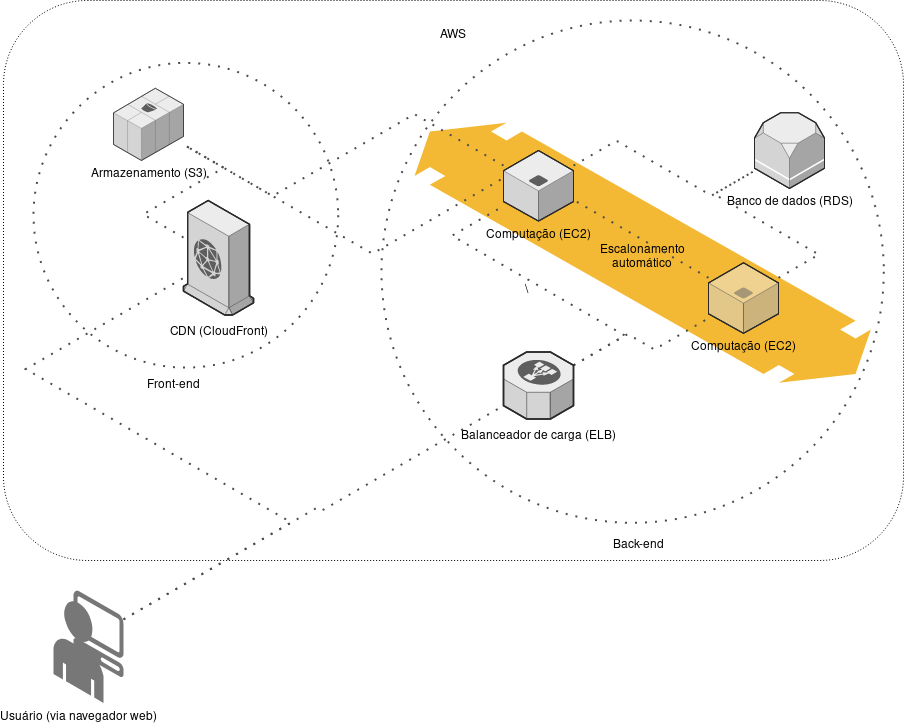
\includegraphics[width=0.8\textwidth]{anexos/arq_fig.png}}
    \fonte{Os autores}
\end{figure}

\subsection{Análise de Requisitos}
    A etapa de análise de requisitos é a parte que os \ac{dt} elaboram as funcionalidades e regras do sistema. Também é definido junto com \ac{po} os requisitos a fim de elaborar as histórias para que esses itens entrem como candidatos para a \emph{\gls{sprint-planning}}. Portanto, os itens são votados na planning para que os \ac{dt} iniciem o desenvolvimento na sprint.
    
\subsubsection{Regras de Negócio}
Foram determinadas dez regras para a nossa plataforma. O \autoref{regra-negocio} contém as \gls{regras-negocio} com seu determinado identificador e a descrição da regra.
\begin{quadro}[H]
	\centering\footnotesize
	\caption{Regras de Negócio}
	\resizebox {.72 \textwidth }{!}{
        \label{regra-negocio}
        \begin{tabular}{|l|p{8cm}|}
        \hline
        \thead{Identificador} & \thead{Descrição} \\ \hline
        RN01 & Os usuários menores de 18 anos não podem realizar o cadastro na plataforma.           
        \\ \hline
        RN02 & Uma vaga publicada pode ficar disponível por até 90 dias, após esse período deve ter opção de renovação ou inativação automática.
        \\ \hline
        RN03 & A exibição de visitas na vaga é exibida em área logada e somente para o perfil família ou agência.
        \\ \hline
        RN04 &  Perfil \emph{au pair}, família e agência podem ser avaliados por comentários e ter a opção de conceder nota, mas não podem se autoavaliar.
        \\ \hline
        RN05 & Somente \emph{au pair} podem receber o consolidado das vagas publicadas nos últimos 7 dias por e-mail.
        \\ \hline
        RN06 & Um \emph{au pair} pode se candidatar em uma ou mais vagas.
        \\ \hline
        RN07 & Família ou agência podem publicar vagas de forma ilimitada.
        \\ \hline
        RN08 & Para cada vaga publicada será cobrado um valor especificado na tabela vigente de preços, considerando se será dado destaque ou não na exibição.
        \\ \hline
        RN09 & Uma família e/ou uma agência podem ter acesso ao publicador.
        \\ \hline
        RN10 & Agência ou família não podem ter acesso aos dados de contatos uma da outra.
        \\ \hline
        \end{tabular}
    }    
\fonte{Autores}
\end{quadro}
    \subsubsection{Requisitos Funcionais}
Durante a etapa de aprofundamento das funcionalidades e de como os recursos do sistema deve se comportar, o projeto requer um maior aprofundamento nas especificações de requisitos para etapa de desenvolvimento, por meio da definição dos \gls{requisitos-funcionais}, a fim de que atenda às necessidades ou expectativas do usuário por meio do comportamento da detecção da execução de funções os quais aparecem com as entradas e saídas, mostrando resultados para a tela do usuário.

A equipe do projeto identificou os requisitos funcionais, os quais são premissas durante o desenvolvimento do projeto, sendo específicos sobre o que o sistema deve entregar, mensuráveis para garantir indicadores de execução, alcançáveis atendendo os prazos do projeto, relevantes para garantir os objetivos do negócio, limitados em seu escopo para possibilitar o acompanhamento do progresso. 
Os requisitos funcionais do projeto foram catalogados e descritos no \autoref{requisitos-funcionais}.



\begin{enumerate}
    \begin{quadro}[H]
    \footnotesize
    \caption{Requisitos Funcionais}
    \label{requisitos-funcionais}
        \begin{tabular}{|p{0.10\linewidth} | p{0.11\linewidth} | p{0.2\linewidth} | p{0.35\linewidth} |}  \hline
          \multicolumn{1}{|c|}{\textbf{Código do Requisito}} &
          \multicolumn{1}{c|}{\textbf{Módulo}} &
          \multicolumn{1}{c|}{\textbf{Nome}} &
          \multicolumn{1}{c|}{\textbf{Descrição}} \\ \hline
          
        REQF01 & Usuário.  &
            Gerenciador de Usuário.                & 
            A aplicação deve permitir que o usuário tenha permissão criar, editar e excluir um usuário. \\  \hline
            
        REQF02 & Login.  &
            Identificar e autenticar com usuário.  &
            A aplicação deve permitir que o usuário realize o acesso em sua conta.                      \\ \hline
            
        REQF03 & Perfil.   &
            Definir perfil de usuário             & 
            A aplicação deve permitir que o usuário defina um perfil (\emph{au pair}, família ou agência).     \\ \hline
            
        REQF04 & Vaga. &
            Gerenciador de anúncio de vaga. 
            & Família ou agência devem poder criar, editar, excluir vagas.                                \\ \hline
            
        REQF05 & Candidatar. &
        Aplicar candidatura em vagas. &
        \emph{Au pair} pode se candidatar a uma ou mais vagas.                                      \\\hline
        REQF06 &
          Favoritos. &
          Salvar vagas em favoritos. &
          \emph{Au pair}, família e agência podem salvar todas as vagas em aberto na lista de favoritos. \\ \hline
          
        REQF07 &
          Consolidado de vagas. &
          Envio do consolidado de novas vagas. &
          \emph{Au pair} tem opção de receber e-mail de consolidado de novas vagas publicadas dos últimos 7 dias.  \\ \hline
          
        REQF08 &
          Filtro de busca. &
          Filtrar perfis de  au pairs, famílias e agências com as melhores avaliações & 
          \emph{Au pair}, famílias e agências devem poder filtrar os perfis melhores avaliados. \\ \hline
          
        REQF09 & 
            Avaliação de perfil. & 
            Os perfis podem avaliar outros perfis & Os perfis devem poder avaliar o perfil de outros usuários.                                  \\ \hline
        REQF10 &
          Priorização de vagas. &
          Vagas com prioridade de visualização. &
          A agência e família devem poder publicar vagas com prioridade de visualização. \\ \hline
          
        \end{tabular}
    \fonte{Autores}
    \end{quadro}
\end{enumerate}

    \subsubsection{Requisitos Não Funcionais}
Com o propósito de especificar as características que o sistema deve conter, define-se os \gls{requisitos-nao-funcionais} que não estão associadas as funcionalidades específicas, sendo que algumas delas não estão perceptíveis para qualquer usuário. 

Aspecto de desempenho da aplicação mediante aos critérios de requisitos mínimos que foram provisionados para o seu funcionamento devendo ser previamente mensurável, a disponibilidade de acesso ao conteúdo das informações da aplicação, quais conteúdos cada usuário pode acessar, portabilidade por meio de fatores do sistema ser adaptável a mudanças, outro fator é a usabilidade da qual o sistema utiliza métodos de controle de acesso, apresentação, estética da interface do usuário, operação e proteção contra erros.

Os requisitos funcionais foram mensurados pela equipe do projeto, o qual buscou enfatizar os controles técnicos visando mitigar riscos relacionados à segurança e garantir escalabilidade e usabilidade, sendo definidos no \autoref{requisitos-nao-funcionais}.
    
    \begin{enumerate}
        \begin{quadro}[H]
        \centering\footnotesize
        \footnotesize
        \caption{Requisitos Não Funcionais}
        \label{requisitos-nao-funcionais}
            \begin{tabular}{|p{0.15\linewidth} | p{0.15\linewidth} | p{0.15\linewidth} | p{0.35\linewidth} |}  \hline
            \multicolumn{1}{|c|}{\textbf{Código do Requisito}} &
              \multicolumn{1}{c|}{\textbf{Módulo}} &
              \multicolumn{1}{c|}{\textbf{Nome}} &
              \multicolumn{1}{c|}{\textbf{Descrição}} \\ \hline
            REQNF01 &
              Usabilidade &
              Usabilidade Sistêmica &
              A aplicação deve conter uma interface desenvolvida para atender a utilização do usuário de forma responsiva \\ \hline
            REQNF02 &
              Performance &
              Escalabilidade de Armazenamento &
              A aplicação deve ser escalável com propósito de suportar aumento e redução de capacidade de armazenamento de dados de acordo com a demanda \\ \hline
            REQNF03 &
              Disponibilidade & Disponibilidade de Dados &
              O provedor dos recursos de hospedagem deve garantir disponibilidade mínima de 95\% ao mês \\ \hline
            REQNF04 &
              Segurança &
              Protocolo de Segurança de dados &
              A aplicação deve conter controle de criptografia TLS ou SSL.  \\ \hline
            REQNF05 &
              Logs &
              Armazenamento de logs &
              A aplicação deve conter logs de transações. \\ \hline
            \end{tabular}
        \fonte{Autores}
        \end{quadro}
    \end{enumerate}

    \subsubsection{Histórias de Usuário}

Em um ambiente ágil, as \ac{histórias de usuário} é um instrumento de escrita utilizado no processo de levantamento de requisitos para descrever a especificação de uma funcionalidade do software, afirmam Beck e Fowler (2001). 

As \ac{histórias de usuário} normalmente seguem o padrão de papel-função-para, onde:\\
•	Como um <tipo de usuário>;\\
•	Gostaria de <algum recurso>;\\
•	Para <alguma razão>.

Para a criação das histórias de usuário utilizaremos o critério de aceitação \ac{bdd}, que significa desenvolvimento orientado por comportamento que se divide em 5 passos, sendo eles: foco em cenário, especificação para o cenário, especificação das unidades, especificação da unidade passar e refatore. 

As \ac{histórias de usuário} que formam nosso \ac{product-backlog} são:

• REQF001 – Usuário (Gerenciador de usuário)
\\ - Quero criar, editar ou excluir uma conta na aplicação;
\\ - Como usuário au pair, família ou agência quero poder criar, editar e excluir a minha conta para ter autonomia sobre minha conta.

• REQF002 – Login (Identificação e autenticação de usuário)
\\ - Quero me autenticar na aplicação;
\\ - Como usuário au pair, família ou agência gostaria de me logar na aplicação para ter acesso às funcionalidades que o sistema disponibiliza.

• REQF003 – Perfil (Definição de perfil de usuário)
\\ - Quero definir meu perfil; 
\\ - Como usuário au pair, família ou agência gostaria de definir meu perfil para ter acesso às funcionalidades da aplicação. 

• REQF004 – Vaga (Gerenciador de anúncios de vaga)
\\ - Quero criar, editar ou excluir anúncios de vagas;
\\ - Como usuário família ou agência gostaria de criar, editar ou excluir anúncios de vagas para obter candidaturas. 

• REQF005 – Candidatar (Aplicar candidaturas)
\\ - Quero me candidatar nas vagas em aberto;
\\ - Como usuário au pair gostaria de me candidatar nas vagas em aberto para o processo de seleção.

• REQF006 – Favoritos (Salvar vagas em favoritos)
\\ - Quero salvar vagas em favoritos;
\\ - Como usuário au pair, família ou agência gostaria de selecionar as vagas em aberto e salvá-las na lista de favoritos para visualizar mais facilmente as vagas que selecionei posteriormente.

• REQF007 – Consolidado de vagas (Envio do consolidado de novas vagas)
\\ - Quero ter a opção de receber o consolidado das novas vagas dos últimos 7 dias;
\\ - Como usuário au pair gostaria de ter a opção de receber e-mail de consolidação de novas vagas publicadas nos últimos 7 dias para me informar sobre as mesmas. 

• REQF008 – Filtro de busca (Filtrar perfis com as melhores avaliações)
\\ - Quero filtrar as agências e famílias com as melhores avaliações.
\\ - Como usuário au pair, família ou agência gostaria de filtrar perfis para encontrar aqueles com as melhores avaliações.

• REQF009 – Avaliação de perfil (Os perfis podem avaliar outros perfis)
\\ - Quero avaliar perfis;
\\-  Como usuário au pair, família ou agência gostaria de opinar sobre o serviço que me foi oferecido para determinar a eficiência e qualidade do serviço prestado ou recebido. 

• REQF010 – Priorização e vagas (Vagas com prioridade de visualização)
\\ - Quero publicar vagas com prioridade de visualização;
\\ - Como usuário agência ou família gostaria de publicar vagas com prioridade de visualização para obter mais atenção dos perfis candidatos para que a vaga seja ocupada em menor tempo.  




    \graphicspath{./anexos}
\subsection{Modelagem}
Com base no escopo apresentado nas seções anteriores a equipe elaborou a modelagem a partir de diagramas \ac{mer} e \ac{der}.

\subsubsection{Modelo Entidade-Relacionamento}
O \ac{mer} exibe detalhes a serem considerados acerca das entidades, atributos e relacionamentos do sistema no momento da projeção do modelo físico, identificando chaves primárias e estrangeiras. Embora o \ac{mer} possa utilizar atributos, o seguinte \ac{mer} não conta com atributos, a fim de proporcionar inicialmente uma visão mais clara do sistema. 
    A \autoref{mer} exibe o \ac{mer}.

\begin{figure}[htb]
    \centering
    \caption{\label{mer}MER}
    \frame{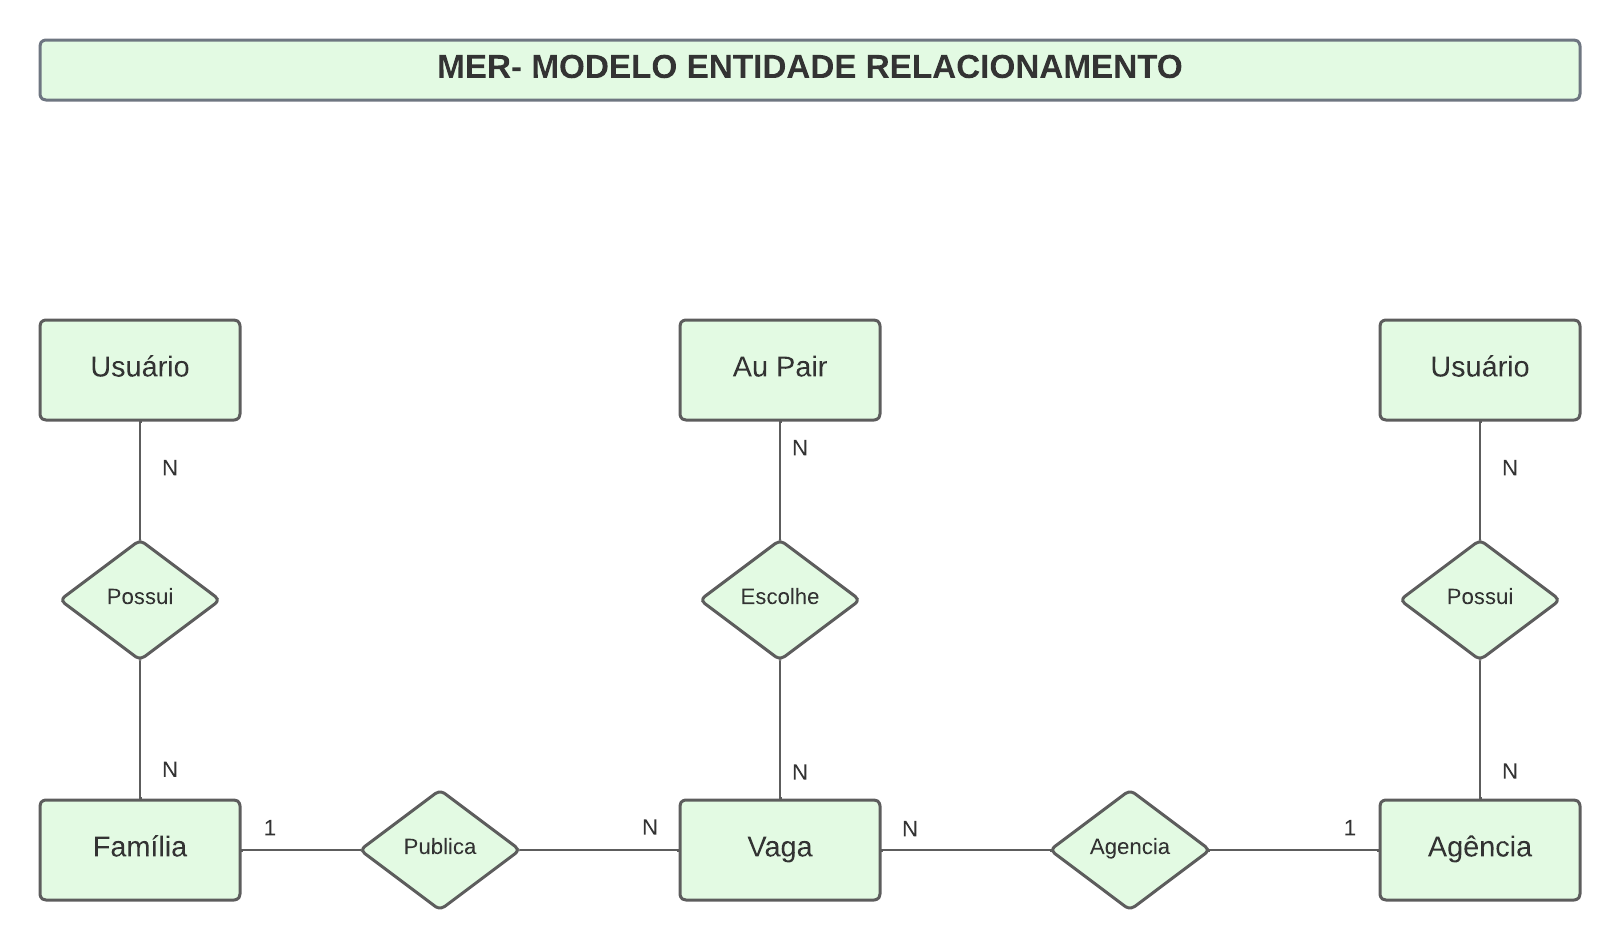
\includegraphics[width=1\textwidth]{anexos/mer.png}}
    \fonte{Autores}
\end{figure}

\subsubsection{Diagrama Entidade-Relacionamento}
Utilizamos o \ac {der} como representação gráfica do \ac{mer}, que apresenta os atributos de cada entidade citada anteriormente no \ac{mer}. O principal objetivo
do \ac{der} é mostrar as estruturas que irão armazenar os dados, e com isso definir melhor as entidades e os seus atributos.

\begin{figure}[H]
    \centering
    \caption{\label{der}DER}
    \frame{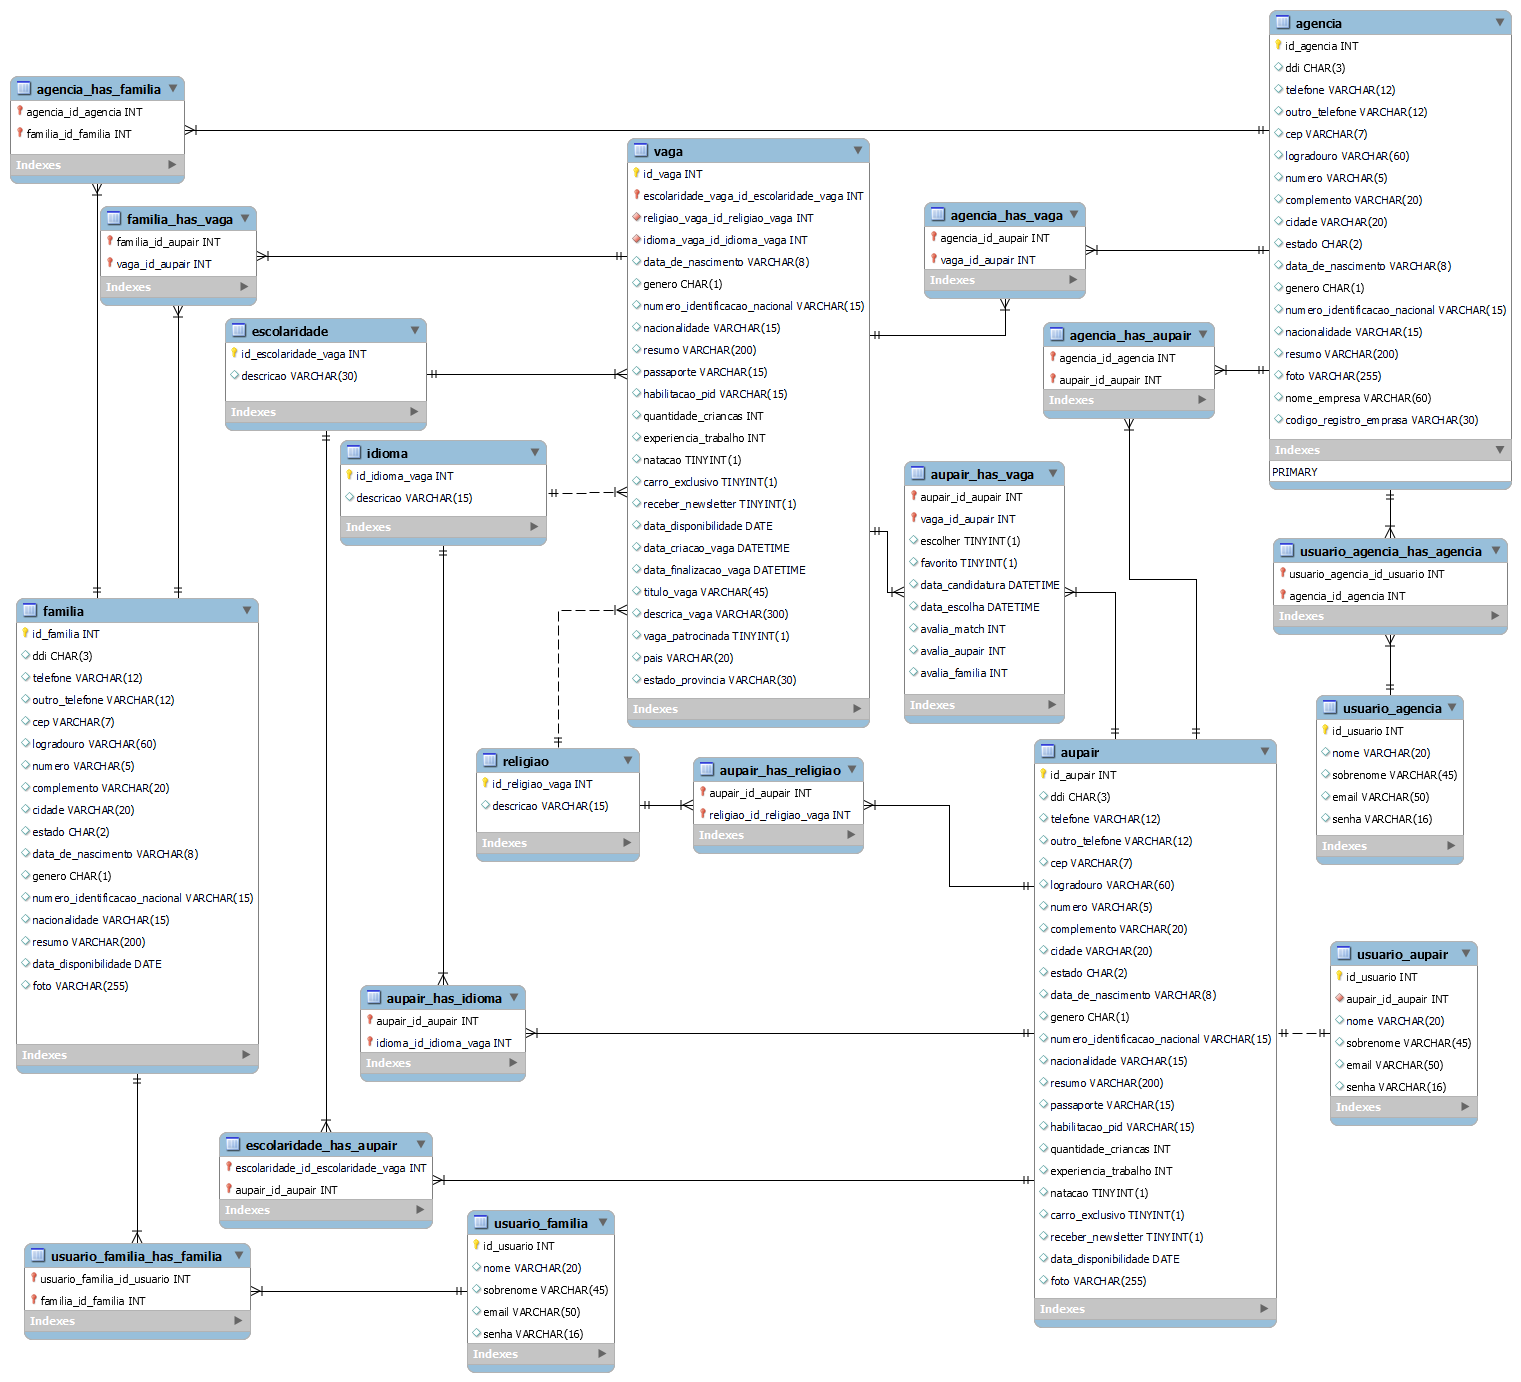
\includegraphics[width=1\textwidth]{anexos/der.png}}
    \fonte{Autores}
\end{figure}

\section{Dicionário de dados}
O dicionário de dados fornece informações adicionais sobre os relacionamentos entre diferentes tabelas de banco de dados além de também ajudar a organizar os dados.

\begin{enumerate}
    \begin{table}[H]
    \caption{Vaga}
    \label{vaga}
    	\centering\footnotesize
        \begin{tabular}{|p{0.40\linewidth} | p{0.04\linewidth} |  p{0.12\linewidth} | p{0.16\linewidth} |}  \hline
        \multicolumn{1}{|c|}{\textbf{Atributos}} &
        \multicolumn{1}{|c|}{\textbf{Chave}} &
        \multicolumn{1}{c|}{\textbf{Descrição}} &
        \multicolumn{1}{c|}{\textbf{Tipo}} \\ \hline
          
        id\_vaga  &  
        PK & 
        Identificador único do registro na tabela de vaga. &
        INT
        \\  \hline
        
        escolaridade\_vaga\_id\_escolaridade\_vaga & 
        FK & 
        Identificador do registro na tabela escolaridade. &
        INT
        \\ \hline
        
       religiao\_vaga\_id\_religiao\_vaga &
       FK &
       Identificador do registro na tabela religiao. &
       INT
       \\ \hline
       
       idioma\_vaga\_id\_idioma\_vaga &
       FK &
       Identificador do registro na tabela idioma. &
       INT
       \\ \hline
       
       data\_de\_nascimento &
       - &
       Data de nascimento. &
       VARCHAR(8)
       \\ \hline
       
       genero &
       - &
       Gênero &
       CHAR(1)
       \\ \hline
       
       numero\_identificacao\_nacional &
       - &
       Número da identidade &
       VARCHAR(15)
       \\ \hline
       
       nacionalidade &
       - &
       Nacionalidade &
       VARCHAR(15)
       \\ \hline
       
       resumo &
       - &
       Resumo &
       VARCHAR(200)
       \\ \hline
       
       passaporte &
       - &
       Passaporte &
       VARCHAR(15)
       \\ \hline
       
       habilitacao\_pid &
       - &
       Permissão internacional para dirigir &
       VARCHAR(15)
       \\ \hline
       
       quantidade\_criancas &
       - &
       Quantidade de crianças &
       INT
       \\ \hline
       
       experiencia\_trabalho &
       - &
       Número de horas de experiência com criança &
       INT
       \\ \hline
       
       natacao &
       - &
       Natação &
       TINYINT(1)
       \\ \hline
       
       carro\_exclusivo &
       - &
       Carro exclusivo para dirigir &
       TINYINT(1)
       \\ \hline
       
       receber\_newsletter &
       - &
       Se deseja receber newsletter &
       TINYINT(1)
       \\ \hline
       
       data\_disponibilidade &
       - &
       Data de disponibilidade &
       DATE
       \\ \hline
       
       data\_criacao\_vaga &
       - &
       Data de criação da vaga &
       DATETIME
       \\ \hline
       
       data\_finalizacao\_vaga &
       - &
       Data de finalização da vaga &
       DATETIME
       \\ \hline
       
       titulo\_vaga &
       - &
       Título da vaga &
       VARCHAR(45)
       \\ \hline
       
       descricao\_vaga &
       - &
       Descrição da vaga &
       VARCHAR(300)
       \\ \hline
       
       vaga\_patrocinada &
       - &
       Se a vaga é pratrocinada &
       TINYINT(1)
       \\ \hline
       
       pais &
       - &
       País &
       VARCHAR(20)
       \\ \hline
       
       estado\_provincia &
       - &
       Estado &
       VARCHAR(30)
       \\ \hline
       
        \end{tabular}
    \fonte{Autores}
    \end{table}
\end{enumerate}

\begin{enumerate}
    \begin{table}[H]
    \caption{regiliao}
    \label{regiliao}
    	\centering\footnotesize
        \begin{tabular}{|p{0.40\linewidth} | p{0.04\linewidth} |  p{0.12\linewidth} | p{0.16\linewidth} |}  \hline
        \multicolumn{1}{|c|}{\textbf{Atributos}} &
        \multicolumn{1}{|c|}{\textbf{Chave}} &
        \multicolumn{1}{c|}{\textbf{Descrição}} &
        \multicolumn{1}{c|}{\textbf{Tipo}} \\ \hline
          
        id\_religiao  &  
        PK & 
        Identificador único do registro na tabela de religiao. &
        INT
        \\  \hline
        
        descricao & 
        - & 
        Descrição &
        VARCHAR(15)
        \\ \hline
       
        \end{tabular}
    \fonte{Autores}
    \end{table}
\end{enumerate}

\begin{enumerate}
    \begin{table}[H]
    \caption{escolaridade}
    \label{escolaridade}
    	\centering\footnotesize
        \begin{tabular}{|p{0.40\linewidth} | p{0.04\linewidth} |  p{0.12\linewidth} | p{0.16\linewidth} |}  \hline
        \multicolumn{1}{|c|}{\textbf{Atributos}} &
        \multicolumn{1}{|c|}{\textbf{Chave}} &
        \multicolumn{1}{c|}{\textbf{Descrição}} &
        \multicolumn{1}{c|}{\textbf{Tipo}} \\ \hline
          
        id\_escolaridade  &  
        PK & 
        Identificador único do registro na tabela de escolaridade. &
        INT
        \\  \hline
        
        descricao & 
        - & 
        Descrição &
        VARCHAR(15)
        \\ \hline
       
        \end{tabular}
    \fonte{Autores}
    \end{table}
\end{enumerate}

\begin{enumerate}
    \begin{table}[H]
    \caption{idioma}
    \label{idioma}
    	\centering\footnotesize
        \begin{tabular}{|p{0.40\linewidth} | p{0.04\linewidth} |  p{0.12\linewidth} | p{0.16\linewidth} |}  \hline
        \multicolumn{1}{|c|}{\textbf{Atributos}} &
        \multicolumn{1}{|c|}{\textbf{Chave}} &
        \multicolumn{1}{c|}{\textbf{Descrição}} &
        \multicolumn{1}{c|}{\textbf{Tipo}} \\ \hline
          
        id\_idioma  &  
        PK & 
        Identificador único do registro na tabela de idioma. &
        INT
        \\  \hline
        
        descricao & 
        - & 
        Descrição &
        VARCHAR(30)
        \\ \hline
       
        \end{tabular}
    \fonte{Autores}
    \end{table}
\end{enumerate}

\begin{enumerate}
    \begin{table}[H]
    \caption{familia\_has\_vaga}
    \label{idioma}
    	\centering\footnotesize
        \begin{tabular}{|p{0.40\linewidth} | p{0.04\linewidth} |  p{0.12\linewidth} | p{0.16\linewidth} |}  \hline
        \multicolumn{1}{|c|}{\textbf{Atributos}} &
        \multicolumn{1}{|c|}{\textbf{Chave}} &
        \multicolumn{1}{c|}{\textbf{Descrição}} &
        \multicolumn{1}{c|}{\textbf{Tipo}} \\ \hline
          
        familia\_id\_vaga  &  
        FK & 
        Identificador único do registro na tabela de vaga &
        INT
        \\  \hline
        
        vaga\_id\_aupair  &  
        FK & 
        Identificador único do registro na tabela de au pair &
        INT
        \\  \hline
       
        \end{tabular}
    \fonte{Autores}
    \end{table}
\end{enumerate}

\begin{enumerate}
    \begin{table}[H]
    \caption{aupair\_has\_vaga}
    \label{idioma}
    	\centering\footnotesize
        \begin{tabular}{|p{0.40\linewidth} | p{0.04\linewidth} |  p{0.12\linewidth} | p{0.16\linewidth} |}  \hline
        \multicolumn{1}{|c|}{\textbf{Atributos}} &
        \multicolumn{1}{|c|}{\textbf{Chave}} &
        \multicolumn{1}{c|}{\textbf{Descrição}} &
        \multicolumn{1}{c|}{\textbf{Tipo}} \\ \hline
          
        aupair\_id\_aupair  &  
        FK & 
        Identificador único do registro na tabela de au pair &
        INT
        \\  \hline
        
        vaga\_id\_aupair  &  
        FK & 
        Identificador único do registro na tabela de au pair &
        INT
        \\  \hline
        
        escolher  &  
        - & 
        Confirmação de candidato selecionado para vaga &
        TINYINT(1)
        \\  \hline
        
        favorito  &  
        - & 
        Vagas favoritas &
        TINYINT(1)
        \\  \hline
        
        data\_candidatura  &  
        - & 
        Data da candidatura &
        DATETIME
        \\  \hline
        
        data\_escolha  &  
        - & 
        Data da escolha da vaga &
        DATETIME
        \\  \hline
        
        avalia\_match  &  
        - & 
        Avaliar o match &
        INT
        \\  \hline
        
        avalia\_aupair  &  
        - & 
        Avaliar au pair &
        INT
        \\  \hline
        
        avalia\_familia  &  
        - & 
        Avaliar familia &
        INT
        \\  \hline
       
       
        \end{tabular}
    \fonte{Autores}
    \end{table}
\end{enumerate}

\begin{enumerate}
    \begin{table}[H]
    \caption{aupair\_has\_religiao}
    \label{idioma}
    	\centering\footnotesize
        \begin{tabular}{|p{0.40\linewidth} | p{0.04\linewidth} |  p{0.12\linewidth} | p{0.16\linewidth} |}  \hline
        \multicolumn{1}{|c|}{\textbf{Atributos}} &
        \multicolumn{1}{|c|}{\textbf{Chave}} &
        \multicolumn{1}{c|}{\textbf{Descrição}} &
        \multicolumn{1}{c|}{\textbf{Tipo}} \\ \hline
          
        aupair\_id\_aupair  &  
        FK & 
        Identificador único do registro na tabela de aupair &
        INT
        \\  \hline
        
        religiao\_id\_religiao\_vaga  &  
        FK & 
        Identificador único do registro na tabela de vaga &
        INT
        \\  \hline
       
        \end{tabular}
    \fonte{Autores}
    \end{table}
\end{enumerate}

\begin{enumerate}
    \begin{table}[H]
    \caption{aupair\_has\_idioma}
    \label{idioma}
    	\centering\footnotesize
        \begin{tabular}{|p{0.40\linewidth} | p{0.04\linewidth} |  p{0.12\linewidth} | p{0.16\linewidth} |}  \hline
        \multicolumn{1}{|c|}{\textbf{Atributos}} &
        \multicolumn{1}{|c|}{\textbf{Chave}} &
        \multicolumn{1}{c|}{\textbf{Descrição}} &
        \multicolumn{1}{c|}{\textbf{Tipo}} \\ \hline
          
        aupair\_id\_aupair  &  
        FK & 
        Identificador único do registro na tabela de aupair &
        INT
        \\  \hline
        
        idioma\_id\_idioma\_vaga  &  
        FK & 
        Identificador único do registro na tabela de vaga &
        INT
        \\  \hline
       
        \end{tabular}
    \fonte{Autores}
    \end{table}
\end{enumerate}

\begin{enumerate}
    \begin{table}[H]
    \caption{familia}
    \label{idioma}
    	\centering\footnotesize
        \begin{tabular}{|p{0.40\linewidth} | p{0.04\linewidth} |  p{0.12\linewidth} | p{0.16\linewidth} |}  \hline
        \multicolumn{1}{|c|}{\textbf{Atributos}} &
        \multicolumn{1}{|c|}{\textbf{Chave}} &
        \multicolumn{1}{c|}{\textbf{Descrição}} &
        \multicolumn{1}{c|}{\textbf{Tipo}} \\ \hline
          
        id\_familia  &  
        PK & 
        Identificador único do registro na tabela de familia &
        INT
        \\  \hline
        
        ddi  &  
        - & 
        Discagem direta internacional &
        CHAR(3)
        \\  \hline
        
        telefone  &  
        - & 
        Telefone &
        VARCHAR(12)
        \\  \hline
        
        outro\_telefone  &  
        - & 
        Telefone &
        VARCHAR(12)
        \\  \hline
        
        cep  &  
        - & 
        CEP &
        VARCHAR(7)
        \\  \hline
        
        logradouro  &  
        - & 
        Logradouro &
        VARCHAR(60)
        \\  \hline
        
        numero  &  
        - & 
        Número &
        VARCHAR(5)
        \\  \hline
        
        complemento  &  
        - & 
        Complemento &
        VARCHAR(20)
        \\  \hline
        
        cidade  &  
        - & 
        Cidade &
        VARCHAR(20)
        \\  \hline
        
        estado  &  
        - & 
        Estado &
        CHAR(2)
        \\  \hline
        
        data\_de\_nascimento  &  
        - & 
        Data de nascimento &
        VARCHAR(8)
        \\  \hline
        
        genero  &  
        - & 
        Gênero &
        CHAR(1)
        \\  \hline
        
        numero\_identificacao\_nacional  &  
        - & 
        Número da identificação &
        VARCHAR(15)
        \\  \hline
        
        nacionalidade  &  
        - & 
        Nacionalidade &
        VARCHAR(15)
        \\  \hline
        
        resumo  &  
        - & 
        Resumo &
        VARCHAR(200)
        \\  \hline
        
        data\_disponibilidade  &  
        - & 
        Data de disponibilidade &
        DATE
        \\  \hline
        
        foto  &  
        - & 
        Foto &
        VARCHAR(255)
        \\  \hline
       
        \end{tabular}
    \fonte{Autores}
    \end{table}
\end{enumerate}

\begin{enumerate}
    \begin{table}[H]
    \caption{usuario\_familia}
    \label{idioma}
    	\centering\footnotesize
        \begin{tabular}{|p{0.40\linewidth} | p{0.04\linewidth} |  p{0.12\linewidth} | p{0.16\linewidth} |}  \hline
        \multicolumn{1}{|c|}{\textbf{Atributos}} &
        \multicolumn{1}{|c|}{\textbf{Chave}} &
        \multicolumn{1}{c|}{\textbf{Descrição}} &
        \multicolumn{1}{c|}{\textbf{Tipo}} \\ \hline
          
        id\_familia  &  
        PK & 
        Identificador único do registro na tabela de usuario\_familia &
        INT
        \\  \hline
        
        nome  &  
        - & 
        Nome &
        VARCHAR(20)
        \\  \hline
        
        sobrenome  &  
        - & 
        Sobrenome &
        VARCHAR(45)
        \\  \hline
        
        email  &  
        - & 
        Email &
        VARCHAR(50)
        \\  \hline
        
        senha  &  
        - & 
        Senha &
        VARCHAR(16)
        \\  \hline
       
        \end{tabular}
    \fonte{Autores}
    \end{table}
\end{enumerate}


\begin{enumerate}
    \begin{table}[H]
    \caption{agencia\_has\_familia}
    \label{idioma}
    	\centering\footnotesize
        \begin{tabular}{|p{0.40\linewidth} | p{0.04\linewidth} |  p{0.12\linewidth} | p{0.16\linewidth} |}  \hline
        \multicolumn{1}{|c|}{\textbf{Atributos}} &
        \multicolumn{1}{|c|}{\textbf{Chave}} &
        \multicolumn{1}{c|}{\textbf{Descrição}} &
        \multicolumn{1}{c|}{\textbf{Tipo}} \\ \hline
          
        agencia\_id\_agencia  &  
        FK & 
        Identificador único do registro na tabela de agencia &
        INT
        \\  \hline
        
        familia\_id\_familia  &  
        FK & 
        Identificador único do registro na tabela de familia &
        INT
        \\  \hline
       
        \end{tabular}
    \fonte{Autores}
    \end{table}
\end{enumerate}


\begin{enumerate}
    \begin{table}[H]
    \caption{agencia\_has\_vaga}
    \label{idioma}
    	\centering\footnotesize
        \begin{tabular}{|p{0.40\linewidth} | p{0.04\linewidth} |  p{0.12\linewidth} | p{0.16\linewidth} |}  \hline
        \multicolumn{1}{|c|}{\textbf{Atributos}} &
        \multicolumn{1}{|c|}{\textbf{Chave}} &
        \multicolumn{1}{c|}{\textbf{Descrição}} &
        \multicolumn{1}{c|}{\textbf{Tipo}} \\ \hline
          
        agencia\_id\_aupair  &  
        FK & 
        Identificador único do registro na tabela de au pair &
        INT
        \\  \hline
        
        vaga\_id\_aupair  &  
        FK & 
        Identificador único do registro na tabela de au pair &
        INT
        \\  \hline
       
        \end{tabular}
    \fonte{Autores}
    \end{table}
\end{enumerate}

\begin{enumerate}
    \begin{table}[H]
    \caption{agencia}
    \label{idioma}
    	\centering\footnotesize
        \begin{tabular}{|p{0.40\linewidth} | p{0.04\linewidth} |  p{0.12\linewidth} | p{0.16\linewidth} |}  \hline
        \multicolumn{1}{|c|}{\textbf{Atributos}} &
        \multicolumn{1}{|c|}{\textbf{Chave}} &
        \multicolumn{1}{c|}{\textbf{Descrição}} &
        \multicolumn{1}{c|}{\textbf{Tipo}} \\ \hline
          
        id\_agencia &  
        PK & 
        Identificador único do registro na tabela de agencia &
        INT
        \\  \hline
        
        ddi  &  
        - & 
        Discagem direta internacional &
        CHAR(3)
        \\  \hline
        
        telefone  &  
        - & 
        Telefone &
        VARCHAR(12)
        \\  \hline
        
        outro\_telefone  &  
        - & 
        Telefone &
        VARCHAR(12)
        \\  \hline
        
        cep  &  
        - & 
        CEP &
        VARCHAR(7)
        \\  \hline
        
        logradouro  &  
        - & 
        Logradouro &
        VARCHAR(60)
        \\  \hline
        
        numero  &  
        - & 
        Número &
        VARCHAR(5)
        \\  \hline
        
        complemento  &  
        - & 
        Complemento &
        VARCHAR(20)
        \\  \hline
        
        cidade  &  
        - & 
        Cidade &
        VARCHAR(20)
        \\  \hline
        
        estado  &  
        - & 
        Estado &
        CHAR(2)
        \\  \hline
        
        data\_de\_nascimento  &  
        - & 
        Data de nascimento &
        VARCHAR(8)
        \\  \hline
        
        genero  &  
        - & 
        Gênero &
        CHAR(1)
        \\  \hline
        
        numero\_identificacao\_nacional  &  
        - & 
        Número da identificação &
        VARCHAR(15)
        \\  \hline
        
        nacionalidade  &  
        - & 
        Nacionalidade &
        VARCHAR(15)
        \\  \hline
        
        resumo  &  
        - & 
        Resumo &
        VARCHAR(200)
        \\  \hline
        
        foto  &  
        - & 
        Foto &
        VARCHAR(255)
        \\  \hline
        
        nome\_empresa  &  
        - & 
        Nome da empresa &
        VARCHAR(60)
        \\  \hline
        
        codigo\_registro\_empresa  &  
        - & 
        Código de registro da empresa &
        VARCHAR(30)
        \\  \hline
       
        \end{tabular}
    \fonte{Autores}
    \end{table}
\end{enumerate}

\begin{enumerate}
    \begin{table}[H]
    \caption{agencia\_has\_aupair}
    \label{idioma}
    	\centering\footnotesize
        \begin{tabular}{|p{0.40\linewidth} | p{0.04\linewidth} |  p{0.12\linewidth} | p{0.16\linewidth} |}  \hline
        \multicolumn{1}{|c|}{\textbf{Atributos}} &
        \multicolumn{1}{|c|}{\textbf{Chave}} &
        \multicolumn{1}{c|}{\textbf{Descrição}} &
        \multicolumn{1}{c|}{\textbf{Tipo}} \\ \hline
          
        agencia\_id\_agencia  &  
        FK & 
        Identificador único do registro na tabela de agencia &
        INT
        \\  \hline
        
        aupair\_id\_aupair &  
        FK & 
        Identificador único do registro na tabela de au pair &
        INT
        \\  \hline
       
        \end{tabular}
    \fonte{Autores}
    \end{table}
\end{enumerate}

\begin{enumerate}
    \begin{table}[H]
    \caption{usuario\_agencia}
    \label{idioma}
    	\centering\footnotesize
        \begin{tabular}{|p{0.40\linewidth} | p{0.04\linewidth} |  p{0.12\linewidth} | p{0.16\linewidth} |}  \hline
        \multicolumn{1}{|c|}{\textbf{Atributos}} &
        \multicolumn{1}{|c|}{\textbf{Chave}} &
        \multicolumn{1}{c|}{\textbf{Descrição}} &
        \multicolumn{1}{c|}{\textbf{Tipo}} \\ \hline
          
        id\_agencia &  
        PK & 
        Identificador único do registro na tabela de usuario\_agencia &
        INT
        \\  \hline
        
        nome  &  
        - & 
        Nome &
        VARCHAR(20)
        \\  \hline
        
        sobrenome  &  
        - & 
        Sobrenome &
        VARCHAR(45)
        \\  \hline
        
        email  &  
        - & 
        Email &
        VARCHAR(50)
        \\  \hline
        
        senha  &  
        - & 
        Senha &
        VARCHAR(16)
        \\  \hline
       
        \end{tabular}
    \fonte{Autores}
    \end{table}
\end{enumerate}

\begin{enumerate}
    \begin{table}[H]
    \caption{agencia\_has\_agencia}
    \label{idioma}
    	\centering\footnotesize
        \begin{tabular}{|p{0.40\linewidth} | p{0.04\linewidth} |  p{0.12\linewidth} | p{0.16\linewidth} |}  \hline
        \multicolumn{1}{|c|}{\textbf{Atributos}} &
        \multicolumn{1}{|c|}{\textbf{Chave}} &
        \multicolumn{1}{c|}{\textbf{Descrição}} &
        \multicolumn{1}{c|}{\textbf{Tipo}} \\ \hline
          
        usuario\_agencia\_id\_usuario  &  
        FK & 
        Identificador único do registro na tabela de usuario\_agencia &
        INT
        \\  \hline
        
        agencia\_id\_agencia &  
        FK & 
        Identificador único do registro na tabela de agencia &
        INT
        \\  \hline
       
        \end{tabular}
    \fonte{Autores}
    \end{table}
\end{enumerate}

\begin{enumerate}
    \begin{table}[H]
    \caption{usuario\_aupair}
    \label{idioma}
    	\centering\footnotesize
        \begin{tabular}{|p{0.40\linewidth} | p{0.04\linewidth} |  p{0.12\linewidth} | p{0.16\linewidth} |}  \hline
        \multicolumn{1}{|c|}{\textbf{Atributos}} &
        \multicolumn{1}{|c|}{\textbf{Chave}} &
        \multicolumn{1}{c|}{\textbf{Descrição}} &
        \multicolumn{1}{c|}{\textbf{Tipo}} \\ \hline
          
        id\_usuario &  
        PK & 
        Identificador único do registro na tabela de usuario\_aupair &
        INT
        \\  \hline
        
        aupair\_id\_aupair  &  
        FK & 
        Identificador único do registro na tabela de aupair &
        INT
        \\  \hline
        
        nome  &  
        - & 
        Nome &
        VARCHAR(20)
        \\  \hline
        
        sobrenome  &  
        - & 
        Sobrenome &
        VARCHAR(45)
        \\  \hline
        
        email  &  
        - & 
        Email &
        VARCHAR(50)
        \\  \hline
        
        senha  &  
        - & 
        Senha &
        VARCHAR(16)
        \\  \hline
       
        \end{tabular}
    \fonte{Autores}
    \end{table}
\end{enumerate}

\begin{enumerate}
    \begin{table}[H]
    \caption{aupair}
    \label{idioma}
    	\centering\footnotesize
        \begin{tabular}{|p{0.40\linewidth} | p{0.04\linewidth} |  p{0.12\linewidth} | p{0.16\linewidth} |}  \hline
        \multicolumn{1}{|c|}{\textbf{Atributos}} &
        \multicolumn{1}{|c|}{\textbf{Chave}} &
        \multicolumn{1}{c|}{\textbf{Descrição}} &
        \multicolumn{1}{c|}{\textbf{Tipo}} \\ \hline
          
        id\_aupair  &  
        PK & 
        Identificador único do registro na tabela de aupair &
        INT
        \\  \hline
        
        ddi  &  
        - & 
        Discagem direta internacional &
        CHAR(3)
        \\  \hline
        
        telefone  &  
        - & 
        Telefone &
        VARCHAR(12)
        \\  \hline
        
        outro\_telefone  &  
        - & 
        Telefone &
        VARCHAR(12)
        \\  \hline
        
        cep  &  
        - & 
        CEP &
        VARCHAR(7)
        \\  \hline
        
        logradouro  &  
        - & 
        Logradouro &
        VARCHAR(60)
        \\  \hline
        
        numero  &  
        - & 
        Número &
        VARCHAR(5)
        \\  \hline
        
        complemento  &  
        - & 
        Complemento &
        VARCHAR(20)
        \\  \hline
        
        cidade  &  
        - & 
        Cidade &
        VARCHAR(20)
        \\  \hline
        
        estado  &  
        - & 
        Estado &
        CHAR(2)
        \\  \hline
        
        data\_de\_nascimento  &  
        - & 
        Data de nascimento &
        VARCHAR(8)
        \\  \hline
        
        genero  &  
        - & 
        Gênero &
        CHAR(1)
        \\  \hline
        
        numero\_identificacao\_nacional  &  
        - & 
        Número da identificação &
        VARCHAR(15)
        \\  \hline
        
        nacionalidade  &  
        - & 
        Nacionalidade &
        VARCHAR(15)
        \\  \hline
        
        resumo  &  
        - & 
        Resumo &
        VARCHAR(200)
        \\  \hline
        
        data\_disponibilidade  &  
        - & 
        Data de disponibilidade &
        DATE
        \\  \hline
        
        foto  &  
        - & 
        Foto &
        VARCHAR(255)
        \\  \hline
       
        \end{tabular}
    \fonte{Autores}
    \end{table}
\end{enumerate}

\begin{enumerate}
    \begin{table}[H]
    \caption{escolaridade\_has\_aupair}
    \label{idioma}
    	\centering\footnotesize
        \begin{tabular}{|p{0.40\linewidth} | p{0.04\linewidth} |  p{0.12\linewidth} | p{0.16\linewidth} |}  \hline
        \multicolumn{1}{|c|}{\textbf{Atributos}} &
        \multicolumn{1}{|c|}{\textbf{Chave}} &
        \multicolumn{1}{c|}{\textbf{Descrição}} &
        \multicolumn{1}{c|}{\textbf{Tipo}} \\ \hline
          
        escolaridade\_id\_escolaridade\_vaga  &  
        FK & 
        Identificador único do registro na tabela de vaga &
        INT
        \\  \hline
        
        aupair\_id\_aupair &  
        FK & 
        Identificador único do registro na tabela de aupair &
        INT
        \\  \hline
       
        \end{tabular}
    \fonte{Autores}
    \end{table}
\end{enumerate}




        \section{Entregáveis por Fase de Entrega}
    O Projeto \textbf{AupaMatch} foi dividido em três grandes fases de entregas, exatamente para corresponder a demanda de produção e validação da aplicação web. As três fases de entregas são: a primeira é a \gls{poc}, a segunda o \gls{mvp} e a última o \textbf{Produto Acabado}. Nas seções seguintes há uma descrição de cada etapa de entrega e o significado desses conceitos.

    \subsection{PoC}
    A \ac{poc} é uma “prova de conceito”, ela serve para que possa ser realizada uma experiência no mercado, porém, sem muita exposição da aplicação web. É a possibilidade de verificar erros e acertos de um software e, assim, se tornar uma evidência da possibilidade de se obter bons resultados no funcionamento.
    Segundo o site do Sebrae a definição do conceito de uma \ac{poc} pode ser descrito como.
    
    \begin{citacao}
        Uma \ac{poc} (Proof of Concept) é a evidência documentada de que um software pode ser bem-sucedido. Ao fazer uma \ac{poc}, é possível identificar erros técnicos que possam interferir no funcionamento e nos resultados esperados. Além disso, a prova de conceito permite a solicitação de \gls{feedbacks} internos e externos. Assim, os testes são realizados sem muita exposição e permite-se a correção de erros e implementação de melhorias.
        \cite{sebrae2018}
    \end{citacao}
    
    A \ac{poc} é a primeira fase das três principais entregas do projeto. Consiste em um protótipo funcional do produto que será entregue. Este protótipo deve ser capaz de demonstrar a funcionalidade do produto e, dessa forma, permitir que seja possível avaliar sua utilidade. Tem-se como objetivo final de uma \ac{poc}, fornecer uma visão clara do produto que está sendo desenvolvido e permitir que seja possível avaliar sua utilidade. Este é um passo importante para garantir que o produto atenda às necessidades e evite futuras rejeições, portanto a \ac{poc} é um conceito que se tornou hoje fundamental no mercado da tecnologia.
        
    \begin{citacao}
        A metodologia de \gls{proof-of-concept} (\ac{poc}) se tornou parte importante do dia a dia de empresas, especialmente das \gls{startups}. Como negócios inovadores e preocupados em lançar produtos que, de fato, resolvam problemas dos seus clientes, é quase indispensável que essas empresas utilizem o \ac{poc} como metodologia em seus processos. \gls{proof-of-concept} (\ac{poc}) é a validação de uma ideia de negócio. Consiste em “tirar a prova” ou validar aquele conceito no mercado. Em outras palavras, trata-se de saber que aquela ideia de produto ou serviço vai encontrar clientes e uma audiência interessada em adquiri-la. Sendo assim, o \ac{proof-of-concept} normalmente é utilizado por empresas pequenas ou \gls{startups} com uma ideia de solução para determinado problema. Naturalmente, é assim que muitas \gls{startups} surgem — elas identificam um problema ou uma dor de determinado grupo de pessoas e criam soluções para resolvê-los.
        \cite{ranDon2022}
    \end{citacao}
    
    \subsection{MVP}
    O \ac{mvp} é a segunda das três principais entregas do projeto.
    Do inglês o \emph{“\ac{minimum-viable-product}”} ou em português Produto Mínimo Viável, trata-se do conjunto mínimo dos elementos necessários para que o produto possa ser levado para produção e possa ser utilizado num cenário real. Seria o momento de validar as ideias, como o próprio nome sugere, esta etapa se refere ao mínimo que é preciso para ter algo viável na produção da aplicação web. 
    É importante definir com a equipe de produção o \ac{mvp} esperado, já que  o objetivo de um \ac{mvp} é fornecer um produto que esteja pronto para o mercado. Uma descrição interessante dessa importante fase poderia ser:
    
    \begin{citacao}
        A ideia por trás do \ac{mvp} é desenvolver uma versão de teste do seu projeto, com o mínimo de investimento financeiro e de tempo, mas capaz de entregar os mesmos valores do produto finalizado. Dessa forma, a ideia pode ser testada e, se aprovada, toda a estrutura necessária para o desenvolvimento é aplicada.
        \cite{rockContent2022}
    \end{citacao}
    
    Portanto, \ac{mvp} Consiste em produtos funcionais que atendam às necessidades esperadas. Este é um passo fundamental para avaliar se o produto está pronto e sem falhas na sua execução além de ser o momento de validação para sua produção final. Outra referência interessante para entender a importância da fase \ac{mvp} é
    
    \begin{citacao}
        É um conjunto de testes primários feitos para validar a viabilidade do negócio. São diversas experimentações práticas que serão desenvolvidas levando o produto a um seleto grupo de clientes… mas não é o produto final! Estamos falando em um produto com o mínimo de recursos possíveis, desde que (em sua totalidade) estes mantenham sua função de solução ao problema para o qual foi criado. Essa técnica de 3 letras ajudou gigantes como \gls{facebook}, \gls{apple} e \gls{dropbox} a se consolidarem em seus segmentos, sem gastarem horrores nos períodos iniciais.
        \cite{endeavor2022}
    \end{citacao}
    

    Consiste em produtos funcionais que atendam às necessidades esperadas. O objetivo de um \ac{mvp} é fornecer um produto que esteja pronto para o mercado. Este é um passo fundamental para avaliar se o produto está pronto e sem falhas na sua execução além de ser o momento de validação para sua produção final.
    
    \subsection{Produto Acabado}
    O Produto Acabado é a terceira e última fase das três principais entregas do projeto. Consiste em produtos finais que atendam às necessidades e expectativas. O produto deve ser capaz de entrar no mercado e gerar receita.
    \section{Critérios de Segurança, Privacidade e Legislação}

O presente capítulo tem por objetivo estabelecer regras a serem observadas no processo de gerenciamento para o desenvolvimento seguro do sistema AupaMatch de forma a possibilitar a inserção da segurança desde a concepção do projeto até a operação, visando a proteção da informação, conformidade com as leis e regulamentos vigentes como a \gls{LGPD} e a disponibilidade do sistema desenvolvido pela WebbStars.  





    \subsection{Segurança dos Dados}

Para a camada de segurança dos dados o sistema AupaMatch deve no mínimo possuir criptografia para dados em transito sendo \gls{TLS} ou \gls{SSL} 3.0 utilizando o protocolo \gls{HTTPS}.

O método \gls{HTTP} Post deve ser utilizado para a transferência de qualquer dado confidencial, e não deve ser utilizado o \gls{Cross-Origin Resource Sharing (CORS)} no sistema.

A aplicação não deve permitir que um usuário não administrador realize a visualização ou modificação de contas de outros usuários.

Deve ser utilizado o bit seguro com a bandeira \gls{HTTP Only} para os \gls{cookies} que contiverem dados sensíveis e confidenciais.

Deve ser utilizado o princípio do privilégio mínimo de acesso e o gerenciamento de usuário pelo administrador da aplicação, sendo inseridos campos com o mínimo de coleta de dados pessoais referente às finalidades e necessidades do negócio.

Devem ser instalados somente os recursos necessários dos \gls{frameworks} de desenvolvimento.
A aplicação deve possuir banco de dados que permita anonimização ou psedoanonimados dos dados pessoais.

Deve ser realizado o gerenciamento dos riscos relacionados a implementação da aplicação.

Qualquer vulnerabilidade identificada no código ou interface da aplicação devem ser corrigidas durante as etapas de desenvolvimento, homologação e produção.

O ambiente deve ser segregado em níveis de desenvolvimento, homologação, pré produção e produção.

Os dados pessoais e dados confidenciais não devem ser processados e armazenados em ambientes de desenvolvimento, homologação e pré-produção.

Todos os softwares utilizados para o desenvolvimento, homologação e produção devem estar licenciados ou atendendo aos requisitos de utilização do software.

Para garantir a proteção contra-ataques de \gls{cross site scripting (XSS)} deve ser realizado a validação de entrada do tipo \gls{whitelist} e codificado todas as informações fornecidas pelo usuário.
    \section{Testes de Segurança}

Os testes de segurança devem ser realizados durante todo o ciclo do desenvolvimento do sistemas, os quais são fundamentais para validação dos requisitos de implementação de controles de segurança, portanto realizar testes desde a concepção do projeto em ambiente de desenvolvimento, homologação e produção do sistema, visa garantir a disponibilidade, integridade e confidencialidade das informações.

A WebbStars utiliza em seu projeto testes baseados no relatório da \gls{OWASP} versão 2021, o qual busca divulgar os maiores tipos e vetores de ataques e suas vulnerabilidades nas aplicações.

\begin{enumerate}
    \begin{quadro}[H]
    \footnotesize
    \caption{Lista OWASP 2021}
    \label{requisitos-funcionais}
        \begin{tabular}{|p{0.04\linewidth} | p{0.40\linewidth} | p{0.50\linewidth} |}  \hline
          \multicolumn{1}{|c|}{\textbf{ID}} &
          \multicolumn{1}{c|}{\textbf{Risco}} &
          \multicolumn{1}{c|}{\textbf{Descrição}}  \\ \hline
    A01& Broken Access Control & O atacante pode escalar privilégios, o que pode levar a descoberta de novas vulnerabilidades.  \\ \hline
    A02 & Cryptographic Failures & O atacante pode acessar ou modificar informações confidenciais. Ex.: cartões de crédito, registros de saúde, dados financeiros (seus ou dos seus clientes).   \\ \hline
    A03 & Injection & É possível roubar a sessão de um usuário, obter dados sensíveis, reescrever a página web, controlar o navegador, redirecionar o usuário para sites de \gls{phishing} ou \gls{malware}.  \\ \hline 
    A04 & Insecure Design & Um design seguro pode ter problemas de implementação que levam a 
    vulnerabilidades que podem ser exploradas, mas um design inseguro não pode ser 
    corrigido por uma implementação perfeita.   \\ \hline
    A05 & Security Misconfiguration & O atacante pode explorar processadores \gls{XML} vulneráveis se puderem fazer upload de XML ou incluir conteúdo hostil em um documento XML, explorando código vulnerável, dependências ou integrações  \\ \hline
    A06 & Vulnerable and Outdated Components & O atacante pode explorar vulnerabilidades contidas em dependências de recursos e bibliotecas. \\ \hline
    A07 & Identification and Authentication Failures & Muitas aplicações acabam falhando no processo de confirmação da identidade do usuário, bem como em processos de autorização, expondo vulnerabilidades e dados de usuários.
\\ \hline
    A08 & Software and Data Integrity Failures & O atacante pode  modificar dados vulneráveis a desserialização insegura.  \\ \hline
    A09 & Security Logging and Monitoring Failures & Registros, detecção, monitoramento e resposta ativa insuficientes podem ocorrer quando. Ex.: Eventos auditáveis, como logins, logins com falha e transações de alto valor não são registrados. \\ \hline
    A10 & Server-Side Request Forgery  & O atacante pode forçar a aplicação a realizar requisições para um domínio arbitrário, permitindo interagir com o servidor e obter informações sensíveis, ocorre porque muitas vezes aplicações buscam recursos remotos sem validar o \gls{URL} fornecido pelo usuário. \\ \hline
        \end{tabular}
    \fonte{Autores}
    \end{quadro}
\end{enumerate}


    \section{Registro e Tratamento de Erros e Falhas}

Qualquer alteração ou transação no sistema devem ser submetidos a coleta e armazenamento de registros, demonstrando como requisitos, quem realizou a alteração, onde foi realizado, quando foi realizado, o que foi alterado ou transacionado.

Em caso de apresentação de um erro, quaisquer dados confidenciais não podem ser expostos sendo: (ID’s de sessão, versão do software, códigos de programação, dados pessoais).

Para qualquer erro deve existir a informação da descrição sem os detalhes do erro em conjunto com o seu código \gls{timestamp}.


    \graphicspath{./anexos}
\section{Tecnologias utilizadas}

\subsection{Front-end}

Se fez necessário a criação de um cliente \gls{spa}, com a biblioteca \ac{React}, visando um menor consumo de recursos do \ac{back-end} e maior dinamismo na experiência de usuário, para além do aproveitamento de código, graças aos componentes que podem ser criados por meio dela. Acrescenta-se o uso do \ac{TypeScript}, objetivando a prevenção de erros de tipagem. A estilização se deu graças ao framework \ac{material}, que fornece classes \ac{css} combinadas para customização de elementos \ac{html}.

\subsection{Back-end}
Para o desenvolvimento do \ac{back-end} do projeto foi utilizado o \ac{node}, o qual foi
escolhido para abarcar as regras de negócio, a migração do banco de dados e fornecimento
da \ac{api}. O banco de dados relacional inicial eleito foi o \ac{MySQL}, mas os membros da equipe possuem mais familiaridade com o \ac{mongodb}. Por isso, optou-se de realizar essa troca.

Por fim, temos o \ac{Nginx} que é usado como proxy reverso, a fim de controlar quais portas e arquivos são disponibilizadas publicamente. 

\subsection{Versionamento, integração contínua e deployment}
O versionamento foi realizado por via da ferramenta \ac{GIT}, e da plataforma de
hospedagem \ac{GitHub}, seguindo o fluxo de trabalho \ac{GitHub Flow}. Através do \ac{GitHub
Actions}, foi feita a execução da integração contínua e montagem (build) da imagem Docker
da aplicação \ac{node}. Inicialmente, foi escolhido o \ac{aws} para as imagens serem carregadas e executada no ambiente, além dos arquivos
estáticos. Mas, como o AWS não possui conexão com o \ac{mongodb}, elegeu-se o \ac{render} para o deploy.
    \section{Modelo de negócio}

Para viabilizar a monetização após a entrega do projeto, o modelo de negócio contará com os planos com acesso às funcionalidades de forma limitada com o plano gratuito e para ter acesso às demais funcionalidade deve ser contratado o plano pago.

\subsection{Planos Gratuito e Pago}

A família, au pair e agência devem ter acesso gratuito à plataforma, contudo existem limitações para o acesso às funcionalidades do sistema. No \autoref{precos-servicos} demonstra todas as funcionalidades que são acessíveis de forma gratuitas e as quais são pagas, sendo que cada um dos perfis tem direito ao acesso. Para as funcionalidades que não são aplicáveis para um determinado perfil estão simbolizados por N/A.


\begin{table}[H]
	\centering\footnotesize
        \caption{Planos Gratuito e Pago}
        \label{precos-servicos}
            \begin{tabular}{|l|c|c|c|c|}
                \hline
                \thead{Funcionalidade}                 & \thead{Au Pair}     & \thead{Família} & \thead{Agência} \\ \hline
                Cadastro de usuário                                & Gratuito       & Gratuito       & Gratuito      \\ \hline
                Filtro de busca de vagas e perfis                      & Gratuito                  & Gratuito       & Gratuito     \\ \hline
                Agenda para disponibilidade de trabalho                & Gratuito             & Gratuito       & Gratuito      \\ \hline
                Alerta de visualização de perfil                    & Gratuito      & Gratuito       & Gratuito           \\ \hline
                Consolidado de vagas                             & Gratuito    & N/A       & N/A        \\ \hline
                Exibição de visitas de vagas                   & Gratuito   & N/A        & N/A       \\ \hline
                Salvar vagas favoritos                   & Gratuito   & N/A       & N/A      \\ \hline 
                Avaliação do perfil   & Gratuito & Gratuito        & Gratuito       \\ \hline
                Consultoria de Carreira por/h  & Pago & N/A        & N/A        \\ \hline
                Apresentação das melhores vagas avaliadas  & Gratuito  & Gratuito        & Gratuito     \\ \hline
                Definir vaga como patrocinada por/vaga  & N/A  & N/A        & Pago     \\ \hline
                Candidatar-se para até 5 vagas de Au Pair por/Mês              & Gratuito             & N/A       & N/A     \\ \hline
                Candidatar-se para mais de 5 vagas Au Pair por/Mês             & Pago            & N/A       & N/A      \\ \hline
                Agenciar vaga  por/unidade              & N/A            & N/A       & Pago      \\ \hline
                Publicador de vaga para Au Pair por/vaga        & N/A             & Pago       & Pago      \\ \hline
            \end{tabular}
\fonte{Autores}
\end{table}

    \section{Viabilidade Financeira}
A análise de viabilidade financeira é importante para qualquer negócio, porque mostra se é possível para uma empresa crescer, quais os riscos envolvidos e se os lucros esperados superam os custos fixos e variáveis.

Em um projeto de desenvolvimento de software, os custos podem ser divididos em dois grandes grupos: os custos fixos e os custos variáveis. Os custos fixos são aqueles que não variam em função do tamanho do projeto, por exemplo, despesas com arrendamento de espaço físico, com aluguel de equipamentos e com mão de obra fixa. Os custos variáveis são aqueles que dependem do tamanho do projeto, como custos com materiais, com mão de obra variável e as despesas com pessoas que trabalham fora do ambiente de desenvolvimento.

\subsection{Análise de Mercado}

Neste cenário de transições digitais onde tudo foi ou vai para internet, entendemos que surge a necessidade de uma ferramenta tecnológica de conexão e intermediação entre au pairs, famílias anfitriãs e as agências de intercâmbio au pair, para gerenciar aspectos no que diz respeito às atividades deste público. A plataforma será desenvolvida para atender a essa necessidade, possibilitando descentralização, promovendo mais transparência, bem como planejamento e ajuste nos objetivos dos envolvidos. 
Dessa forma, o AupaMatch, além de contribuir com os interessados, gerencia as informações relacionadas.
    \subsection{Custos do Projeto}

Os custos para o desenvolvimento do projeto estão detalhados para viabilizar o esclarecimento entre as partes interessadas para aceitação e provisão de investimentos para o projeto, o qual deve consumir os recursos financeiros e tempo investidos em cada uma das etapas que forem iniciadas no projeto, sendo eles: 

\begin{itemize}
    \item Fase 1 - Planejamento;
    \item Fase 2 - Desenvolvimento;
    \item Fase 3 - Entrega e Validação;
\end{itemize}

Realizadas uma análise de mercado sobre o custo empregatício dos profissionais de tecnologia da informação na cidade de São Paulo, a WebbStars relaciona os custos do projeto a carga de horas trabalhadas pelos profissionais envolvidos, o qual está detalhado na \autoref{custo-projeto-horas-trabalhadas}, sendo referência o recurso empregado em cada uma das fases do projeto, a quantidade de horas para as entregas, custo por horas trabalhadas e horas utilizadas do profissional.

\begin{enumerate}
    \begin{quadro}[H]
    \caption{Custo de Horas Trabalhadas por Profissional}
    \label{custo-projeto-horas-trabalhadas}
    	\centering\footnotesize
        \begin{tabular}{|p{0.40\linewidth} | p{0.04\linewidth} | p{0.10\linewidth} |  p{0.08\linewidth} | }  \hline
        \multicolumn{1}{|c|}{\textbf{Recurso}} &
        \multicolumn{1}{|c|}{\textbf{Qntd.}} &
        \multicolumn{1}{c|}{\textbf{H/BRL}} &
        \multicolumn{1}{c|}{\textbf{Horas}} \\ \hline
          
        {\textbf{Fase 1 - Planejamento}}    &   &    &          \\  \hline
        Analista de Segurança & 0 & 78,2 & 0            \\ \hline
        Analista de Infraestrutura & 0 & 55,55 & 0         \\ \hline
        Analista de Desenvolvimento de Sistemas & 2 & 72,84 & 18              \\ \hline
        Analista de testes &  0 &  53,46 & 0                              \\\hline
        Analista de Treinamento &  0 &  50,00 & 0                          \\\hline
            & &  & \\ \hline
       {\textbf{Fase 2 - Desenvolvimento}}    &   &    &          \\  \hline
        Analista de Segurança & 1 & 78,2 & 30            \\ \hline
        Analista de Infraestrutura & 0 & 55,55 & 0         \\ \hline
        Analista de Desenvolvimento de Sistemas & 5 & 72,84 & 190              \\ \hline
        Analista de testes &  1 &  53,46 & 30                              \\\hline
        Analista de Treinamento &  0 &  50,00 & 0                          \\\hline
            & &  & \\ \hline
       {\textbf{Fase 3 - Entrega e Validação}}    &   &    &         \\  \hline
        Analista de Segurança & 1 & 78,2 & 16            \\ \hline
        Analista de Infraestrutura & 1 & 55,55 & 26         \\ \hline
        Analista de Desenvolvimento de Sistemas & 1 & 72,84 & 6             \\ \hline
        Analista de testes &  0 &  53,46 & 0                              \\\hline
        Analista de Treinamento &  1 &  50,00 & 10                          \\\hline   
        \end{tabular}
    \fonte{Autores}
    \end{quadro}
\end{enumerate}

Os custos por etapa e os custos totais do projeto estão detalhados na \autoref{custo-projeto} o qual demonstra pelas fases do projeto, quantidade de horas trabalhadas dos profissionais envolvidos e o custo de cada entrega e fase.

\begin{enumerate}
    \begin{quadro}[H]
    \caption{Custos do Projeto}
    \label{custo-projeto}
    	\centering\footnotesize
        \begin{tabular}{|p{0.60\linewidth} | p{0.04\linewidth} | p{0.10\linewidth} | }  \hline
        \multicolumn{1}{|c|}{\textbf{Fases do Projeto}} &
        \multicolumn{1}{c|}{\textbf{Horas}} &
        \multicolumn{1}{c|}{\textbf{BRL}} \\ \hline
          
        {\textbf{Fase 1 - Planejamento}}    & 18 &  {\textbf{2.622,24}}               \\  \hline
        Levantamento de Necessidades  e Requisitos de Negócio & 6 & 874,08             \\ \hline
        Desenvolvimento do Plano de Projeto & 6 & 874,08           \\ \hline
        Desenvolvimento do Plano de Comunicação e Atividades & 6 & 874,08              \\ \hline
        Aprovação de Orçamento e Plano de Projeto &  - &  -                              \\\hline
            & &   \\ \hline
        {\textbf{Fase 2 - Desenvolvimento}} & & {\textbf{73.048,20}} \\ \hline
        Preparação para Desenvolvimento & 30 & 10.926,00   \\ \hline
        Desenvolvimento e Adaptações & 100 & 36.420,00   \\ \hline
        Testes Funcionais e Segurança & 30 & 14.776,20  \\ \hline
        Documentação do Projeto & 60 & 10.926,00   \\ \hline
             & &  \\ \hline
        {\textbf{Fase 3 - Entrega e Validação}} & 68 & {\textbf{4.183,24}}  \\ \hline
        Implantação e Homologação p/Ambiente de Produção & 30 & 1.665,00\\ \hline
        Testes de Segurança & 16 & 1.251,20\\ \hline
        Treinamento interno & 10& 500,00\\ \hline
        Operação assistida & 6 & 330,00\\ \hline
        Desenvolvimento History Book & 6 & 437,04\\ \hline
        Aceitação do Cliente e encerramento & - & -\\ \hline
        & & \\ \hline
        {\textbf{Custo Total do Projeto}} &  & {\textbf{79.953,28}}\\ \hline        
        \end{tabular}
    \fonte{Autores}
    \end{quadro}
\end{enumerate}
    \subsection{Custos Operacionais}

Após a entrega definitiva do projeto, a operação do sistema AuPairMatch deve ser iniciada, contudo os custos fixos foram apresentados na \autoref{custos-fixos} e os custos variáveis na \autoref{custos-variaveis}, os quais são relevantes para compor o faturamento final da operação mensal.

\begin{enumerate}
    \begin{quadro}[H]
    \caption{Custos do Fixos}
    \label{custos-fixos}
    	\centering\footnotesize
        \begin{tabular}{|p{0.30\linewidth} | p{0.10\linewidth} | {0.10\linewidth} | p{0.10\linewidth} | p{0.10\linewidth} |}  \hline
        \multicolumn{1}{|c|}{\textbf{Custo}} &
        \multicolumn{1}{|c|}{\textbf{USD}} &
        \multicolumn{1}{|c|}{\textbf{Câmbio}} &
        \multicolumn{1}{|c|}{\textbf{BRL}} &
        \multicolumn{1}{|c|}{\textbf{BRL + IOF}} \\ \hline
          

    Analista de Suporte (10h/Mês) & N/A & N/A & 1.000,00 & 1.000,00 \\ \hline
    Contabilidade & N/A & N/A & 500,00 & 500,00 \\ \hline
    Amazon CDN CloudFront (1TB Gratuíto) & - & 5,30 & - & - \\ \hline 
    Amazon EC2 & 64,54 & 5,30 & 342,00 & 363,82 \\ \hline
    Amazon RDS for MySQL & 34,97 & 5,30 & 195,41 & 204,60 \\ \hline
    Amazon Simple Storage Service (S3) & 51,12 & 5,30 & 270,94 & 288,23 \\ \hline
    Elastic Load Balancing & 36,87 & 5,30 & 195,41 & 207,88 \\ \hline
    Imposto ISS  & - & - & - & - \\ \hline
    Imposto PIS/Pasep & - & - & - & -\\ \hline
    Imposto Cofins & - & - & - & - \\ \hline
    
         {\textbf{Custo Fixo Mensal Total}}   &    & & &   {\textbf{2.564,53}}           \\  \hline 

        \end{tabular}
    \fonte{Autores}
    \end{quadro}
\end{enumerate}


\begin{enumerate}
    \begin{quadro}[H]
    \caption{Custos Variáveis Mensal}
    \label{custos-variaveis}
    	\centering\footnotesize
        \begin{tabular}{|p{0.50\linewidth} | p{0.11\linewidth} | p{0.2\linewidth} | p{0.35\linewidth} |}  \hline
        \multicolumn{1}{|c|}{\textbf{Custo}} &
          \multicolumn{1}{c|}{\textbf{BRL}} \\ \hline
          
                & \\ \hline

        Serviços de Suporte Técnico de TI (5h/mês) & 500,00           \\ \hline
        Serviços de Advocacia & 500,00                     \\ \hline
        Propaganda/Anúncios Mensais & 2000,00                \\\hline

        & \\ \hline
        {\textbf{Custo Variável Mensal Total}} & {\textbf{3.000,00}}\\ \hline        
        \end{tabular}
    \fonte{Autores}
    \end{quadro}
\end{enumerate}
    \subsection{Preços dos Serviços}

Os serviços e os seus respectivos preços são cobrados por acesso às funcionalidades específicas por unidade e em moeda Dólar Americano USD, os quais foram mensurados e estão definidos na  \autoref{precos-servicos}.

\begin{quadro}[H]
	\centering\footnotesize
        \caption{Preços dos Serviços}
        \label{precos-servicos}
            \begin{tabular}{|l|c|c|c|c|}
                \hline
                \thead{Funcionalidade}                 & \thead{AuPair}     & \thead{Família} & \thead{Agência} \\ \hline
                Cadastro de usuário                                & Gratuito       & Gratuito       & Gratuito      \\ \hline
                Filtro de busca de vagas e perfis                      & Gratuito                  & Gratuito       & Gratuito     \\ \hline
                Agenda para disponibilidade de trabalho                & Gratuito             & Gratuito       & Gratuito      \\ \hline
                Alerta de visualização de perfil                    & Gratuito      & Gratuito       & Gratuito           \\ \hline
                Consolidado de vagas                             & Gratuito    & N/A       & N/A        \\ \hline
                Exibição de visitas de vagas                   & Gratuito   & N/A        & N/A       \\ \hline
                Salvar vagas favoritos                   & Gratuito   & N/A       & N/A      \\ \hline 
                Avaliação do perfil   & Gratuito & Gratuito        & Gratuito      \\ \hline
                Apresentação das melhores vagas avaliadas  & Gratuito  & Gratuito        & Gratuito     \\ \hline
                Vaga patrocinada por/publicação  & N/A  & N/A        & 5,00     \\ \hline
                Candidatar-se para até 5 vagas de AuPair por/Mês              & Gratuito             & N/A       & N/A     \\ \hline
                Candidatar-se para mais de 5 vagas AuPair por/Mês             & 5,00            & N/A       & N/A      \\ \hline
                Agenciar vaga  por/unidade              & N/A            & N/A       & 50,00      \\ \hline
                Publicador de vaga para Au Pair por/vaga        & N/A             & 20,00       & 20,00      \\ \hline
            \end{tabular}
\fonte{Autores}
\end{quadro}


    \subsection{Faturamento Projetado}

O faturamento projetado é a somatória de todos os custos fixos e variáveis totais subtraídos pela somatória de receitas totais com a venda de serviços, o faturamento projetado realista o qual apresenta o cenário razoável para o sistema AuPairMatch está detalhado na \autoref{faturamento-projetado-realista}, o faturamento projetado otimista o que apresenta o melhor cenário estimado está descrito no \autoref{faturamento-projetado-otimista}, e o faturamento projetado pessimista o que apresenta o pior cenário está descrito no \autoref{faturamento-projetado-pessimista}.

\begin{enumerate}
    \begin{quadro}[H]
    \caption{Faturamento Projetado Realista}
    \label{faturamento-projetado-realista}
    	\centering\footnotesize
        \begin{tabular}{|p{0.50\linewidth} | p{0.04\linewidth} |  p{0.10\linewidth} |}  \hline

        \multicolumn{1}{|c|}{\textbf{RECEITAS PREVISTAS}} &
        \multicolumn{1}{|c|}{\textbf{QTD.}} &
        \multicolumn{1}{|c|}{\textbf{BRL}} \\ \hline


    Consultoria de Carreira por/h   & 20 & 1.590,00         \\ \hline
    Definir vaga como patrocinada por/vaga  & 5 & 132,50      \\ \hline
    Candidatar-se para mais de 5 vagas AuPair por/Mês     &  15 & 412,50     \\ \hline
    Agenciar uma vaga             &  10  & 2.650,00          \\ \hline
    Publicador de vaga para Au Pair por/vaga     & 50  &   5.300,00     \\ \hline
    {\textbf{Faturamento Total}}   &   &   {\textbf{8.415,00}}           \\  \hline 


    &   &        \\ \hline
    \multicolumn{1}{|c|}{\textbf{DESPESAS PREVISTAS}} &
    \multicolumn{1}{|c|}{\textbf{QTD.}} &
    \multicolumn{1}{|c|}{\textbf{BRL}} \\ \hline

    Amazon CDN CloudFront (1TB Gratuíto) & - & 0 \\ \hline 
    Amazon EC2 & - & 363,82\\ \hline
    Amazon RDS for MySQL & - & 204,60 \\ \hline
    Amazon Simple Storage Service (S3) & - & 288,23 \\ \hline
    Elastic Load Balancing & - & 207,88 \\ \hline
    Contabilidade & - & 500,00 \\ \hline
    Analista de Suporte para plataforma (h/Mês) & 10 & 417,60  \\ \hline
    Imposto ISS 2\% sobre a receita bruta & - & 168,30  \\ \hline
    Imposto PIS/Pasep-faturamento 0,65\% & - & 54,70  \\ \hline
    Imposto Cofins-faturamento 3\% & - & 252,45  \\ \hline
    Propaganda/Anúncios Mensal    & - &  2.000,00  \\ \hline
    
    
    {\textbf{Despesas Totais}}   &   &   {\textbf{4.457,58}}           \\  \hline 


        & &   \\  \hline   
    {\textbf{Lucro Líquido}}   &   &   {\textbf{3.957,42}}           \\  \hline 

        \end{tabular}
    \fonte{Autores}
    \end{quadro}
\end{enumerate}

\begin{enumerate}
    \begin{quadro}[H]
    \caption{Faturamento Projetado Otimista}
    \label{faturamento-projetado-otimista}
    	\centering\footnotesize
        \begin{tabular}{|p{0.50\linewidth} | p{0.04\linewidth} |  p{0.10\linewidth} |}  \hline

        \multicolumn{1}{|c|}{\textbf{RECEITAS PREVISTAS}} &
        \multicolumn{1}{|c|}{\textbf{QTD.}} &
        \multicolumn{1}{|c|}{\textbf{BRL}} \\ \hline


    Definir vaga como patrocinada por/vaga  & 10 & 265,00      \\ \hline
    Candidatar-se para mais de 5 vagas AuPair por/Mês     &  30 & 825,00     \\ \hline
    Agenciar uma vaga             &  20  & 5.300,00         \\ \hline
    Publicador de vaga para Au Pair por/vaga     & 100  &   10.600,00     \\ \hline
    {\textbf{Faturamento Total}}   &   &   {\textbf{16.990,00}}           \\  \hline 


    &   &        \\ \hline
    \multicolumn{1}{|c|}{\textbf{DESPESAS PREVISTAS}} &
    \multicolumn{1}{|c|}{\textbf{QTD.}} &
    \multicolumn{1}{|c|}{\textbf{BRL}} \\ \hline

    Amazon CDN CloudFront (1TB Gratuíto) & - & 0 \\ \hline 
    Amazon EC2 & - & 363,82\\ \hline
    Amazon RDS for MySQL & - & 204,60 \\ \hline
    Amazon Simple Storage Service (S3) & - & 288,23 \\ \hline
    Elastic Load Balancing & - & 207,88 \\ \hline
    Contabilidade & - & 500,00 \\ \hline
    Analista de Suporte para plataforma (h/Mês) & 10 & 417,60  \\ \hline
    Imposto ISS 2\% sobre a receita bruta & - & 339,80  \\ \hline
    Imposto PIS/Pasep-faturamento 0,65\% & - & 110,43  \\ \hline
    Imposto Cofins-faturamento 3\% & - & 509,7  \\ \hline
    Propaganda/Anúncios Mensal    & - &  4.000,00  \\ \hline
    
    
    {\textbf{Despesas Totais}}   &   &   {\textbf6.942,06}}           \\  \hline 


        & &   \\  \hline   
    {\textbf{Lucro Líquido}}   &   &   {\textbf{10.047,94}}           \\  \hline 

        \end{tabular}
    \fonte{Autores}
    \end{quadro}
\end{enumerate}

\begin{enumerate}
    \begin{quadro}[H]
    \caption{Faturamento Projetado Pessimista}
    \label{faturamento-projetado-pessimista}
    	\centering\footnotesize
        \begin{tabular}{|p{0.50\linewidth} | p{0.04\linewidth} |  p{0.10\linewidth} |}  \hline

        \multicolumn{1}{|c|}{\textbf{RECEITAS PREVISTAS}} &
        \multicolumn{1}{|c|}{\textbf{QTD.}} &
        \multicolumn{1}{|c|}{\textbf{BRL}} \\ \hline


    Definir vaga como patrocinada por/vaga  & 3 & 79,50      \\ \hline
    Candidatar-se para mais de 5 vagas AuPair por/Mês     &  8 & 220,00     \\ \hline
    Agenciar uma vaga             &  5  & 1325,00          \\ \hline
    Publicador de vaga para Au Pair por/vaga     & 25  &   2.650,00     \\ \hline
    {\textbf{Faturamento Total}}   &   &   {\textbf{4.274,50}}           \\  \hline 


    &   &        \\ \hline
    \multicolumn{1}{|c|}{\textbf{DESPESAS PREVISTAS}} &
    \multicolumn{1}{|c|}{\textbf{QTD.}} &
    \multicolumn{1}{|c|}{\textbf{BRL}} \\ \hline

    Amazon CDN CloudFront (1TB Gratuíto) & - & 0 \\ \hline 
    Amazon EC2 & - & 363,82\\ \hline
    Amazon RDS for MySQL & - & 204,60 \\ \hline
    Amazon Simple Storage Service (S3) & - & 288,23 \\ \hline
    Elastic Load Balancing & - & 207,88 \\ \hline
    Contabilidade & - & 500,00 \\ \hline
    Analista de Suporte para plataforma (h/Mês) & 10 & 417,60  \\ \hline
    Imposto ISS 2\% sobre a receita bruta & - & 85,49  \\ \hline
    Imposto PIS/Pasep-faturamento 0,65\% & - & 27,80  \\ \hline
    Imposto Cofins-faturamento 3\% & - & 128,25  \\ \hline
    Propaganda/Anúncios Mensal    & - &  300,00  \\ \hline
    
    
    {\textbf{Despesas Totais}}   &   &   {\textbf{2.523,67}}           \\  \hline 


        & &   \\  \hline   
    {\textbf{Lucro Líquido}}   &   &   {\textbf{1.750,83}}           \\  \hline 

        \end{tabular}
    \fonte{Autores}
    \end{quadro}
\end{enumerate}
    \subsection{Retorno sobre o Investimento}

A expectativa de retorno sobre o investimento \gls{ROI} realizado está projetado para ocorrer após a implementação do sistema, e início da etapa de operacionalização, sendo necessário considerar os cumprimentos das metas de lucros estabelecidos em cada período de fechamento do faturamento operacional considerando aspectos de volatilidade e sazonalidade.

A WebbStars detalhou os cenário de alcance total do indicador do \gls{ROI} para o projeto AuPairMarch na \autoref{roi}, considerando o cenário de faturamento realista, otimista e pessimista de retorno do investimento para o investidor.

\begin{enumerate}
    \begin{table}[H]
    \caption{Custos Variáveis Mensal}
    \label{roi}
    	\centering\footnotesize
        \begin{tabular}{|p{0.40\linewidth} | p{0.10\linewidth} | p{0.10\linewidth} |}  \hline
        \multicolumn{1}{|c|}{\textbf{Custo}} &
          \multicolumn{1}{c|}{\textbf{BRL}} &
         \multicolumn{1}{c|}{\textbf{Meses}}   \\ \hline

        Faturamento Projetado Realista & 3957,42 & 21          \\ \hline
        Faturamento Projetado Otimista & 10.047,94 &  8                \\ \hline
        Faturamento Projetado Pessimista & 1.750,83 &  44                           \\\hline

        \end{tabular}
    \fonte{Autores}
    \end{table}
\end{enumerate}
   
    \chapter{Links do Projeto}
    \begin{figure}[htb]
\caption{\label{qr-url-2}QR code com Blog do projeto}
\begin{center}
\qrcode[height=2.4cm]{https://webbstarsifspgrupo1.blogspot.com/}
\legend{\url{https://webbstarsifspgrupo1.blogspot.com/}}
\end{center}
\end{figure}

\begin{figure}[htb]
\caption{\label{qr-url-2}QR code com Canal do Youtube}
\begin{center}
\qrcode[height=2.4cm]{https://www.youtube.com/channel/UCfDRS-cEblV_HnaLMBvlerA/featured}
\legend{\url{https://www.youtube.com/channel/UCfDRS-cEblV_HnaLMBvlerA/featured}}
\end{center}
\end{figure}

\begin{figure}[htb]
\caption{\label{qr-url-2}QR code com Link do Projeto no GitHub}
\begin{center}
\qrcode[height=2.4cm]{https://github.com/WebbStars}
\legend{\url{https://github.com/WebbStars}}
\end{center}
\end{figure}

\begin{figure}[htb]
\caption{\label{qr-url-2}QR code com Repositório no SVN do IFSP}
\begin{center}
\qrcode[height=2.4cm]{https://svn.spo.ifsp.edu.br/svn/a6pgp/S202202-PI-NOT/WebbStars/}
\legend{\url{https://svn.spo.ifsp.edu.br/svn/a6pgp/S202202-PI-NOT/WebbStars/}}
\end{center}
\end{figure}

    
    % ---
% Conclusão (outro exemplo de capítulo sem numeração e presente no sumário)
% Dependendo do trabalho desenvolvido ele pode ter uma Conclusão ou Considerações finais
% Para trabalhos de disciplina utilizar Considerações Finais
% ---
\chapter{Considerações Finais}
% Exemplo de como adicionar linha adicional no sumário
%\addcontentsline{toc}{chapter}{Considerações Finais}
% Para definir sem número utilizar o asterisco
% Mas se tiver sub seção vai continuar a contagem do capítulo anterior
%\chapter{Considerações finais}



% ---
Além desse documento ser um modelo de como pode ser criado um documento em \LaTeX \space ele também apresenta diversas informações úteis para as disciplinas de projetos de informática do \ac{ifsp} e alguns elementos uteis para as monografias do curso de Pós Graduação em Gestão de \acs{ti} do \ac{ifsp}.

\explicacao{Um trabalho de disciplina não tem \enquote{Conclusão}}

\preencheComTexto


\explicacao{Exemplo de possíveis seções para monografia da pós graduação...}
\section{Resposta à Questão de Pesquisa}
\preencheComTexto

\section{Objetivos Propostos}
\preencheComTexto

\section{Contribuições Acadêmicas e Gerenciais}
\preencheComTexto

\section{Limitações da Pesquisa e Contribuições para Estudo}
\preencheComTexto

    
    \bibliography{referencias,capitulo/abntex2-doc-abnt-6023}
    
    %%% INCLUIR QUANDO NECESSÁRIO OU NO FINAL DO TRABALHO %%%
    % ----------------------------------------------------------
% Glossário
% ----------------------------------------------------------
%
\ifdef{\printnoidxglossary}{
    \addcontentsline{toc}{chapter}{GLOSSÁRIO}
    \printnoidxglossary[style=glossario]
    %\printglossaries
}{}
    %% ----------------------------------------------------------
% Apêndices
% Documentos gerados pelo próprio autor
% ----------------------------------------------------------

% ---
% Inicia os apêndices
% ---
\begin{apendicesenv}

% Imprime uma página indicando o início dos apêndices
\partapendices

% ----------------------------------------------------------
\chapter{Quisque libero justo}
% ----------------------------------------------------------

\preencheComTexto

% ----------------------------------------------------------
\chapter{Nullam elementum urna vel imperdiet sodales elit ipsum pharetra ligula
ac pretium ante justo a nulla curabitur tristique arcu eu metus}
% ----------------------------------------------------------
\preencheComTexto

\end{apendicesenv}
% ---

    %% ----------------------------------------------------------
% Anexos
% Documentos gerados por outros autores
% ----------------------------------------------------------

% ---
% Inicia os anexos
% ---
\begin{anexosenv}
\anexos
% Imprime uma página indicando o início dos anexos
\partanexos

% ---
\chapter{Manual todonotes(parcial)}
\label{manual-todonotes}
% ---
\index{pdf}
% se pages = "-"  fica com arquivo completo
\includepdf[pages=1-3,scale=0.8,frame=true,pagecommand={}]{anexos/todonotes.pdf}

% ---
% Para incluir sem gerar a quebra de página inicial no anexo
\includepdf[pages=1,scale=0.7,frame=true,pagecommand=\chapter{Manual pdfpages(parcial)}\label{manual-pdfpages}]{anexos/pdfpages.pdf}
\includepdf[pages=2-3,scale=0.8,frame=true,pagecommand={}]{anexos/pdfpages.pdf}

% ---
\chapter{Manual acronym(parcial)}
\index{pdf}
% somente algumas páginas para exemplo sem borda
\includepdf[pages=1-3,frame=false,pagecommand={}]{anexos/acronym.pdf}



\includepdf[frame=true,scale=0.7,pagecommand=\chapter{Referência Rápida pifont}\label{pifont-quickref}]{anexos/pifont.pdf}


\end{anexosenv}

    
    
    %---------------------------------------------------------------------
    % INDICE REMISSIVO - Quando necessário 
    % As palavras indexadas devem ser definidas com \index{} no texto
    %---------------------------------------------------------------------
    \phantompart

    %---------------------------------------------------------------------
\end{document}